\chapter{AUTONOMOUS MORPHOLOGY AS A TARGET OF LEARNING}
\label{autonomous}

%Or (Toward) Learning Morphology By Itself
%%%%%%%%%%%%%%%%%%%%%%%%%%%%%%%%
%% The main point of this chapter is the following: "It's not implausible to 
%% take a non-morpheme-based approach, to assume that morphology
%% is independent of phonology and syntax." Put another way, the main goal
%% is to justify taking a non-morpheme-based approach.
%%
%% This justification will mainly involve pointing out that many scholars
%% argue for autonomous morphology in one way or another. I will basically
%% be citing precedents. These the authors of the "Word-and-Paradigm" (WP) camp.
%% Aronoff is in this group, but he is not the only one. Who else? Whom shall describe
%% in some depth, and whom shall I merely mention in passing? In passing: Anderson,
%% Mathews, [Network morphology], ...
%% In some depth: Stump, Aronoff
%% However, most WP proponents these days, assume that Aronoff's morphomes exist.
%% and use the term morphome in their own theories.
%Where the \ac{ULM}  
%``Unsupervised Learning of Morphology" is concerned, what 
%is the learning target? The most immediate answer would 
%seem to be ``morphology,"
%
%but this answer would be ambiguous. You see...
%If one should ask a few linguists to summarize over the 
%meaning of \emph{morphology}
%of \emph{morphology}.
%One of the most pernicious 
%[and yet potentially most solvable] 
%problems in \ac{ULM} 
%%the Unsupervised Learning of 
%%Morphology (\ac{ULM} ) 
%is that its researchers do not seem to understand what
%their systems are learning. That is, morphological status
%what
%their systems
\section{Introduction}
Many morphologists in recent decades have rejected the notion of the morpheme---a concept that inextricably binds morphology to syntax and semantics---in favor of approaches that regard morphology as autonomous, i.e., as independent 
of both syntax/semantics and phonology. The principle objective of this chapter is to 
%\begin{itemize}
%\item 
show that autonomous morphological units are legitimate learning targets for a \ac{ULM}  system. In fact, as we shall soon, autonomous morphology is more than just legitimate; it is the only possible learning target for \ac{ULM}  as it is conventionally defined. %, i.e., to show that it makes sense to try to learn morphological units that are not morphemes.
%\item 
In the course of the discussion, we shall consider some of the more prominent theories of autonomous morphology, contrasting them with ``non-automonous" approaches, and  noting their significance to \ac{ULM} (and Multimorph in particular).

%and discuss their signifance where relationship to \ac{ULM}  and, more specifically, to Multimorph.
%\end{itemize}
% is to demonstrate that autonomous morphology is more than as a earning target for a \ac{ULM}  system. However, autonomous morphology, as we shall see, is more   in doing so, we shall  But more than that, this chapter will show , %an unsupervised morphological learning system, 
%instead to develop\emph{autonomous morphology} refers to a view of morphology wherein morphology is considered to be independent of both syntax/semantics and phonology.  often used to describe morphological theories 
%The main objective of this chapter is to demonstrate that not only is autonomous morphology


\section{The Unsupervised Learning of \textit{What}, Exactly?} 
In the \ac{ULM} literature, authors often use the word \emph{morpheme(s)} 
when describing their the systems' \emph{learning target(s)}, i.e., what their systems are meant to learn and 
output, as well as the features that compose their input feature vectors.
\cite{poon-et-al:2009}, for example, use two main categories 
of features, one of which they refer to as \emph{morpheme-context} features (see ch. REF).
\cite{goldsmith:2001, goldsmith:2006} also uses the word 
\emph{morpheme}.
%The word \emph{morpheme} is often present in the very titles of papers, e.g., 
%``Unsupervised Discovery of Morphemes" \citep{creutz-and-lagus:2002} and 
%``Unsupervised Models for Morpheme Segmentation and Morphology 
%Learning" \citep{creutz-and-lagus:2007}, 
%both titles by the creators of Morfessor \citep{creutz-and-lagus:2002, 
The creators of Morfessor 
\citep{creutz-and-lagus:2002, 
creutz-and-lagus:2005, creutz-and-lagus:2007}
%They also use \emph{morpheme} in the text of their papers, e.g.,
use a range of terms, including 
\emph{morpheme},
\emph{morpheme-like}, and \emph{morph}. The following quotations 
illustrate these usages (emphasis added):
\begin{exe}
\ex ``The model presented in this 
work provides a good means for the segmentation of words into 
\textbf{morphemes} \citep[][p. 6]{creutz-and-lagus:2007}. 
\ex``[W]e have demonstrated how the meaning and form of 
\textbf{morpheme-like} units can be modeled in a 
morphology induction task\dots" \citep{creutz-and-lagus:2005}.
\ex``The lexicon contains one entry for each distinct \textbf{morph} 
(morph type) in the 
segmented corpus" \citep[][p. 9]{creutz-and-lagus:2007}. 
\end{exe}
Creutz and Lagus seem to prefer the more general, theory-neutral term \emph{morph} 
in more formal or technical contexts. Indeed,
of the above three terms, they probably use 
\emph{morph} most frequently.

Moreover, \ac{ULM} researchers virtually never specify what they mean
when they use the word \emph{morphology}, even though there
are currently at least two fundamentally different schools of thought concerning the nature of morphology. These are the 
the \emph{morpheme-based} and \emph{lexeme-based} views, to borrow the labels that \cite{aronoff:1994} has assigned 
to these categories. The lexeme-based view, to which a majority of morphologists now subscribe (CITE),
maintain that there exists an \emph{autonomous} layer of morphology, a layer that mediates between (morpho-)syntax
and phonological realization, but has neither meaning nor phonologically realized form in and of itself. Proponents
of lexeme-based morphology thus do not believe in pairings of form and meaning, i.e., morphemes, as fundamental linguistic
units. We shall further discuss the notion of autonomous morphology in section (REF). 

One's morphological theory effects the way in which one interprets the output of a \ac{ULM}  system. 
If one describes a \ac{ULM}  system and its learning task in terms of 
morpheme-based morphology, one must also struggle to 
describe its output as consisting of morphemes, as do, for example, 
\cite{creutz-and-lagus:2007,creutz-and-lagus:2005}. In contrast, under a 
lexeme-based theory, one would view the output of a \ac{ULM}  system as 
consisting of \emph{autonomous} morphological units, i.e., 
expressly non-morpheme units. 
Thus, one's theory of morphology makes an implicit claim about the output of 
his/her \ac{ULM}  system.
%At this point, the attentive reader would be well-justified 
%in asking, 
%``WTF? What the F-word does Morfessor learn? What indeed 
%does \emph{any} 
%\ac{ULM}  system learn?" Indeed, dear reader, these are 
%excellent questions; 
%they will prove very significant to us, particularly the latter, 
%more general question, for it is directly relevant to what we 
%expect Multimorph is to learn.

The output of any machine learning system depends to 
a great extent on the nature of its input, which, in the case of the 
\emph{unsupervised} learning of morphology, 
depends on with the meaning of ``unsupervised to a large extent." 
%In the case of \ac{ULM} , the input is invariably a list of contextless words [cite?]. 
%And thus no syntactic or otherwise word-external features can be considered. 
%Any categories acquired by the algorithm thus cannot be conventional (or ``classical") 
%%morphemes, since morphemes are by definition minimal pairings of form and meaning.
%Now unsupervised learning is of course central to \ac{ULM} , 
%but one might might reasonably ask what ``unsupervised" 
%means in the context of morphological learning. 
All of the major \ac{ULM}  
systems take as input a list of independent tokenized words (CITE).
Thus, a convention seems to have emerged whereby, in the 
case of \ac{ULM} , the meaning of \emph{unsupervised} includes a
requirement that each word be free of morphosyntactic 
or semantic information. In practice,
this means being entirely free of context. I am 
not aware of a \ac{ULM}  system that extracts features from a word's raw context, i.e.,
unanalyzed adjacent words. Presumably, this is because 
such a context would not be helpful to a machine learner. 
It would probably have to be abstracted and categorized 
(i.e., annotated) in order
for it to be helpful to a system. 
%The word underanalysis is help a system makes of the given unanalyzed 
%word in question.
%sequence of symbols, completely lacking in external information. 
%There is neither context nor annotation of any kind, and no thus 
%means of inducing semantics, i.e., of pairing forms with their 
%functions. 

Because morphemes are irreducible and arbitrary pairings of form and meaning
but in order to deduce meaning, one needs contextual information. Because
a \ac{ULM} system does not have access to context, it simply cannot learn classical morphemes.
A \ac{ULM} system might learn subsequences of word strings that happen to resemble
 classical morphemes \emph{in form}, but only because there is always morphological systems do 
 tend to cooperate with syntax/semantics in some way, and in some cases this cooperation appears more transparent and straightforward than
 in others.  However, this \ac{ULM} system 
 would nevertheless be oblivious to what
 these pieces of form actually mean. Meaning is an essential component of the classical morpheme, and because
 meaning depends on context, there is no way to induce classical morphemes from contextless words.
%Since the words input to a \ac{ULM system are not accompanied by contextual features,
%there is no way to induce classical morphemes from contextless words, as meaning, which is determined by context, is 
%is an essential component of the classical morpheme.
%\footnote{Bloomfield, the leader of the American 
%Structuralists, provided the following early definition of the 
%\emph{morpheme}: ``[A] morpheme is a recurrent 
%(meaningful) form which cannot in 
%turn be analyzed into smaller recurrent (meaningful) forms. 
%Hence any unanalyzable word or formative is a morpheme" 
%\citep[][p. 155]{bloomfield:1926}.} 
Therefore, \ac{ULM} systems, particularly those which learn solely from 
from lists of raw, contextless words, simply cannot learn 
\emph{morphemes} in the strict sense of the term.

Consider, for example, Linguistica, the seminal 
\ac{ULM}  system developed by \cite{goldsmith:2001, goldsmith:2006}. 
Linguistica finds morphological relationships by filling in 
data structures 
called \emph{signatures} as it iterates over datasets comprising many
thousands of contextless words. Each signature $\sigma$ 
comprises 
two sets, $S$ and $A$, a set of stems and a set of affixes, 
respectively %, and is defined with respect to
%a corpus $C$. In particular, $\sigma= (S, A)$ if and only if
%\begin{itemize}
%   \item $S$ contains at least two stems, and $A$ at least two affixes.
%   \item Every stem in $S$ appears in $C$ with every affix in $A$. That is, every combination in $S \times A$ must be attested
%   in $C$, %That is, if $S = \{ s_1,s_2,s_3 \}$
%  % and $A = \{ a_1,a_2 \}$, then 
%   where $S \times A$ comprises $s_1 a_1$, $s_1 a_2$, $s_2 a_1$, $s_2 a_2$, $s_3 a_1$, and $s_3 a_2 $.
%\end{itemize}
A \emph{signature} is a pair of sets, namely a set of stems $S$ and 
a set of affixes $A$, such that each stem-affix combination in the cross 
product $S \times A$ is observed in the corpus. Additionally, $S$ and 
$A$ must each contain at least two members, with \textsc{null} being 
a permissible member, and each stem can belong to only one signature.  
%Crucially, each stem must occur in the corpus with each affix.  and likewise, each of the affixes must have been seen with each of the stems; 
%otherwise, the two sets do not constitute a signature.
%Given a tokenized corpus of words $W$, a \emph{signature} is a pairing of two sets, a set of stems $S$ and a set of affixes $A$, such that every stem-affix combination in $S \times A$ is attested in $W$; i.e., $S \times A \subseteq W$. Furthermore, $S$ and $A$ must each contain at least two members.
For example, a signature could be the following $S = \{ \text{act}, \text{back}, \text{mint} \}$ 
and $A = \{ \textsc{null}, \text{s}\}$. Every possible stem-affix combination is 
\begin{equation}
\label{eq:SxA}
S \times A = \{ \text{act}, \text{back}, \text{mint}, \text{act-s}, 
\text{back-s}, \text{mint-s}\}
\end{equation}
The fifth 
most common signature that Linguistica found among the words of 
\textit{Tom Sawyer} had as its affix set $\{\textsc{null}\textit{.ed.ing.s}\}$  \cite{goldsmith:2001}. 
%It corresponding stem set had 14 members. 
%\footnote{Its corresponding
%stem component had 14 members, but the identities of these stems are not given.}
%but
%the paper is the affix component in one of 
%the signatures that  Linguistica has extracted from the words of the novel \textit{Tom Sawyer}. 
The corresponding stem set had 14 members, though \cite{goldsmith:2001} 
does not identify the individual stems. 
In any case, the affix set \textsc{null}\textit{.ed.ing.s} represents 
a stem equivalence class. Its extraction would be an impressive achievement for any \ac{ULM}  system, and this
is but one of many such signatures that Linguistica has found. However, 
suppose we had no knowledge of English. It would then be impossible to deduce the nature 
of this equivalence class. We might
guess that it is a morphosyntactic category of \emph{some kind}, but since we would be ignorant
of the affixes' meanings/functions, this would be nothing more than a guess. 
%It would be entirely beyond our reach to attempt to guess the type of
%morphosyntactic category.
%We certainly could not begin to posit a particular morphosyntactic category.

An English speaker can probably deduce that \textsc{null}\textit{.ed.ing.s} are suffixes that attach to verbs,
but this it is the speaker's general competence in the language that informs this deduction, not anything in the 
signatures themselves. 
%[These stems were verbs clearly the nullsoft facts attached to the base case 
%the e d direct past tense the ing corresponds to the progressive or the present 
%participle in the s the third person singular present tense suffix.] 
%Now, it is not hard to guess the lexical category of the stems that accompany \textsc{null}\textit{.ed.ing.s}. 
%Clearly these are verbal suffixes.
%But it is not 
%But an English speaker would know this only because he/she know that \textsc{verb} + \textit{-ed} realizes a
%past-tense verb, \textsc{verb} + \textit{-s} realizes a 3rd-person 
%singular present-tense
%verb, and so on. 

Thus, although Linguistica does learn morphological equivalence classes, 
sets of stems that combine with the same affixes 
(and sets of affixes that combine with with the same stems) 
it does not learn to associate \textit{-s}, for example, 
with `3rd-person singular present-tense'. That is, it does not assign particular
meanings to the stems and affixes it discovers.
Nor would Linguistica know the particular meaning of any stem 
associated with a given affix set. 
Suppose that \{\textit{act}, \emph{jump}, and \emph{laugh}\} 
were the stem set associated with \textsc{null}\textit{.ed.ing.s}. 
Linguistica would thus have learned that these stems are the same 
in a way. But Linguistica would not have learned what this 
equivalence should have signified, not would have learned the semantic 
distinctions between the members of the same equivalence set. 
That is, even though \textit{act}, \emph{jump}, and \emph{laugh} 
share the same affix set, they do not share the same meaning. 
Thus, we must conclude that Linguistica does not learn morphemes 
in the classical sense, i.e., with each morpheme being a
pairing of one form and one meaning.

To be sure, this is not a failing on the 
part of Linguistica, which is indeed an effective 
unsupervised learner of morphology. Given the definition 
of the classical morpheme and the limited nature of 
Linguistica's input, it is simply not possible for 
Linguistica to learn true morphemes. First, because 
Linguistica is an \emph{unsupervised} learner, it has 
no access to the information it would need to assign 
%meanings to forms, as discussed above. Second, according to 
%many morphologists, morphemes do not adequately 
%account for the full range of morphological
%phenomena. Indeed, for these morphologists, morphemes do not exist.
Second, as we shall see in section~\ref{sec:morpho-theories}, morphemes do not adequately 
account for the full range of morphological phenomena \citep{anderson:2017}. 
For these reasons, morphemes are not reasonable 
targets of unsupervised morphological learning.
%do not even exist in the first place. 
 %the \emph{meaning} of \textit{act}, e.g., 
% that \emph{act} and
%\emph{jump} and \emph{laugh} do not share the same meaning, even though they (might) share
%the same affix set. Linguistica thus does not learn morphemes.
%We would then know each one means, include how it functions, i.e., how it interacts 
%(or does not interact with other morphemes). 
%For example, if know what \textit{act} and {-ed} mean individually, then we know, at 
%least according to the morpheme-based view of morphology, then we know what 
%and what \textit{act-ed} means, namely `act, \textsc{past-tense}'


%----------------------------------------
%Thus, Goldsmith?s signatures are clever devices for extracting meaning from raw, unannotated text. 
%\begin{enumerate}
%\item the nature of the algorithm 
%\item learns depends of course on the nature 
%\end{enumerate}
%of the algorithm, and there is wide variety of unsupervised learning algorithms out there.
%way in which these algorithms can be we (and on the nature of the input), 
%but in any case, the output of any \ac{ULM}  system will consist of forms entirely or almost entirely and be virtually void 
%of any real meaning. 
%It will find units that are building blocks of a sort, but these building blocks may not be what one expects. 
%They will serve to account for the internal structure of words while remaining utterly blind to the external contexts 
%might coincide the elements of word-internal structure. \citep{stump:2012}.

%\section{But if Not Morphemes, What?}
\section{A Spectrum of Morphological Theories}
\label{sec:morpho-theories}
%While Linguistica may learn morphology,  This is clearly apparent in 
%its signatures. % are clearly morphological structures.
%, I must say that it is an impressive system.
In the preceding section, we argued that Linguistica does not learn morphemes. The same can be said of Morfessor, 
the system of \cite{poon-et-al:2009}, and %virtually
%(if not absolutely) all 
every other \ac{ULM}  system. 
%but not morphemes, even though
% the word morpheme was used by Goldsmith.
 % the word morpheme. The Morfessor bunch at least seems to demonstrate some awareness that Morfessor 
%does not learning morphemes, using words like X and Y, yet even they use the word morpheme often enough.
 But how can we say that these systems learn morphology, but not morphemes? As it turns out,
 the existence of morphemes is by no means a sure thing.  
 %Many theories of morphology have been proposed over the last 1.2 million years. 
%are two opposing views in morphology. 
 %One believes in morphemes, the does not. 
 %However, these many theories, like so many tiny flakes of iron, have been drawn to one or the other of  two antithetical poles.
 %These camps have been described characterized in various ways.

\subsection{Stump's Taxonomy of Morphological Theories}
%%\subsubsection{Stump's Taxonomy of Morphological Theories}
\cite{stump:2001}'s oft-cited taxonomy of morphological theories 
consists of four categories. These four arise from two independent 
binary distinctions, namely \emph{lexical} vs. \emph{inferential} on the hand, and \emph{incremental} vs. \emph{realizational} on the other.
%In other words, anyone who is strongly considering formulating a new morphological theory has two overarching decisions to make, each corresponding to one of the binary distinctions. The first is whether the theory is 
%to be \emph{lexical} or \emph{inferential}. The second decision, which is orthogonal the first, is whether the theory is to be \emph{incremental} of \emph{realizational}.
%\begin{enumerate}
%   \item Decisition \emph{lexical} or \emph{inferential}? 
%   \item Is it \emph{incremental} or \emph{realizational}? 
%\end{enumerate}
%We might call the first decision the``\textsc{meaning source}" 
%decision and the second ``\textsc{direction}."  
%Consider for instance 
%the plural noun \textit{issues}. Suppose it is our morphologist's view that
%the meaning of \textit{issue+s} stems directly from the 
%meanings of the entries for \textit{issue} and \textit{-s} in the lexicon.
%She would then choose \emph{lexical} over \emph{inferential}. 
%But if she should instead believe that the meaning of 
%\textit{issue+s} is due to a rule like ``\textit{X+s} 
%is the plural form of \textit{X}," inferred from analogous forms like \textit{dog+s} and \textit{bike+s},
%she would then choose \textit{inferential} 
%instead of \emph{lexical}.
 
%As for the second decision, she would choose \emph{incremental} if she believes that 
%a word's meaning is built up as it acquires affixes; in others words, that the meaning of depends on its affixes
%  On the other hand, if she believed
%that a word's meaning determines its form and licenses a particular set
%of morphology exponents, she will
%choose \emph{realizational}. In 
\begin{exe}
\ex \textsc{First Distinction}: \textit{Lexical vs. Inferential} %(\citet{stump:2001}'s first distinction) \label{ex:d-one} 
\begin{xlist}
	\ex \textbf{Lexical}: The meaning of \textit{issue-s}, for example, is determined by the lexical entries of its components \textit{issue} and \textit{-s}.
%	  of the meanings of its components, which are specified in the lexicon. means what it does because its components, particularly /+s/, e mean what they do. as simply the composition of two lexical entries. 
%namely those for \textit{issue} and \textit{-s}. affixes, along with stems (for both are morphemes) have entries in the lexicon, and morphosyntactic properties are part of a morpheme's lexical entry. \label{ex:d-one-a}
	\ex \textbf{Inferential}: The meaning of \textit{issue-s} is determined by the meanings of related forms like \textit{dog-s} and \textit{bike-s},
%``treat morphological structure as grounded in the relations between classes of words" \citep[][p. 2]{anderson:2015shorthist}. %sim of form reflecting sim of content directly? The meaning of 
%In other words, %a form like
%\textit{issue+s} means what it does
%%, namely `\textit{issue} + \textsc{singular},'  
%because related forms like \textit{dog+s} and \textit{bike+s} mean what they do, 
with ``similarities of form [directly] reflecting similarities of content and vice versa" \citep[][p. 2]{anderson:2015shorthist}. \label{ex:d-one-b}
	\end{xlist}
\ex \textsc{Second Distinction}: \textit{Incremental vs. Realizational} %(\citet{stump:2001}'s second distinction) \label{ex:d-two} 
\begin{xlist} 
	\ex \textbf{Incremental}: Each affix has its own intrinsic meaning. 
	A form's \ac{MPS} is thus built up incrementally as it acquires affixes.
%	Thus, if an affix is removed from a word, the affix's meaning is also removed.  Conversely, whenever an affix is added to a form, the form's semantics ``annexes," as it were, the meaning of the affix (cf. the work of Ren\'e de Saussure). 
	\label{ex:d-two-a}
	\ex \textbf{Realizational}: A word's set of morphosyntactic properties 
	licenses a particular configuration of morphological exponents 
	(i.e., usually affixes of some sort). 
	%and thus realizes the phonological form. \label{ex:d-two-b}
	\end{xlist}
\end{exe}

%The two choices for the first decision are:
%\begin{description} 
%\item[Lexical:] The meaning of \textit{issue+s} is simply the composition of two lexical entries. 
%namely those for \textit{issue} and \textit{-s}. affixes, along with stems (for both are morphemes) have entries in the lexicon, and morphosyntactic properties are part of a morpheme's lexical entry.
%%She would then choose \emph{lexical} over \emph{inferential}.
%\item[Inferential theories] 
%``treats morphological structure as grounded in the relations between classes of words" \citep[][p. 2]{anderson:2015shorthist}. %sim of form reflecting sim of content directly? The meaning of 
%For example, the form 
%\textit{issue+s} means what it does, namely '\textit{issue} + \textsc{plural}'  because related forms like \textit{dog+s} and \textit{bike+s} mean what the they do, with ``similarities of form [directly] reflecting similarities of content and vice versa" (ibid.)
%%the rule ``\textit{X+s} 
%%is the plural form of \textit{X}," which is inferred from analogous forms like 
%%\textit{dog+s} and \textit{bike+s}.
%\end{description}
%The two choices for the second decision are:
%\begin{description}
%\item[Incremental:] Each affix has its own local meaning. Thus, if an affix is removed from a word, the innate meaning of the affix is also removed.  in the affix. Conversely, whenever an affix is added to a form, the form's semantics ``annexes," as it were, the meaning of the affix (cf. the work of Ren\'e de Saussure). 
%%final meaning depends on which affixes were added to it.
%\item[Realizational:] The meaning of a word, i.e., its set of morphosyntactic properties, determines its form. That is, the morphosyntactic properties invoke a rule that assembles the a particular group of morphological exponents.
%
%\emph{licenses} a particular set of exponents.
%\end{description}

By cross-combining the options of first distinction with those of the second, 
\cite{stump:2001} derives four categories of morphological theories. 
\emph{Lexical-Incremental} and \emph{Lexical-Realizational} theories 
on the one hand, and on the other, \emph{Inferential-Incremental} and 
\emph{Inferential-Realizational} theories. However, \citep{anderson:2017} 
notes that most theories fall into the \emph{Lexical-Incremental} and 
\emph{Inferential-Realizational} categories. Indeed, these are the two are 
the most extreme of the four categories in that they are entirely antithetical. 
The ongoing debate over the nature and status of morphology can largely 
be framed in terms of the opposition between these two categories. 

The distinction between \emph{Lexical-Incremental} 
and \emph{Lexical-Realizational} 
theories is essentially the same as the distinction 
that \cite{aronoff:1994} draws
between \emph{morpheme-based} and \emph{lexeme-based} 
views of morphology. Morpheme-based approaches regard 
the classical morpheme as the seat of meaning. %These are the legacy of Bloomfield and the descriptivists.
The concept of the morpheme and morpheme-centered morphological analysis
was developed by Bloomfield in the 1920s and 1930s 
\citep{bloomfield:1926, bloomfield:1933} and honed by his 
successors in the descriptivist program, e.g., % \cite[e.g.,][]{hocket:1947, harris:1955}.
\cite{hockett:1947} and \cite{harris:1955}.
It was \cite[][p. 161]{bloomfield:1933} who famously wrote, ``A linguistic form 
which bears no partial phonetic-semantic resemblance to any other form is a \emph{simple} form or \emph{morpheme}" (emphasis in the original). 
%\citep[][p. 161]{bloomfield:1933}.
%a distinct, irreducible pairing of form and meaning.  
That is, a morpheme, as a pairing of a form and a meaning, is a fundamental unit; it cannot be analyzed into smaller units
of form and meaning.
Moreover, Bloomfield and the descriptivists maintained that
each \emph{complex form}, i.e., each word comprising 
two or more morphemes, was \emph{exhaustively decomposable} 
into morphemes. That is, every phonological segment
in a given word had to be either a morpheme or part of a morpheme. 


%  ``Thus [A] morpheme is a recurrent (meaningful) form which cannot in turn be analyzed into smaller recurrent (meaningful) forms. Hence any unanalyzable word or formative is a morpheme" \cite[][p. 155]{bloomfield:1926}. It was Leonard Bloomfield, founder of descriptivism,  linguistic form which bears no partial phonetic-semantic resemblance to any other form is a \emph{simple} form or \emph{morpheme}." \citep[][p. 161]{bloomfield:1933}. Moreover, according to Bloomfield, every word comprises one or more morphemes, and every word must be \emph{exhaustively decomposable} into morphemes. That is, every phonological segment in a given word must either be a morpheme or part of morpheme. The concept of the morpheme and morpheme-centered morphological analysis
%was developed by Leonard Bloomfield \cite{bloomfield:1926, bloomfield:1933} and honed by his 
%descriptivist successors. 

The influence of Bloomfield and the descriptivists %(or American structuralists)
cannot be easily underestimated. Bloomfieldian concepts and methods 
pervade introductory linguistics courses and textbooks, both at
the undergraduate and graduate level. Any introductory text containing 
a unit on morphological analysis is going to present a methodology that 
is essentially Bloomfieldian \citep{anderson:2017}.
% morphological unit in an introductory linguistics textbook
%ccourse on morphology or general linguistics course teaches essentially 
%Bloomfieldian methods of morphological analysis. The morpheme is central concept in any undergraduate
%linguistics textbook. 
It is therefore perhaps no surprise that
computational linguists, including researchers in the field of \ac{ULM}, 
tend to presume %a morpheme-based morphology.
the reality of Bloomfieldian morphemes and the soundness of a 
Bloomfieldian view of morphology. The Bloomfieldian approach is essentially
the lexical-incremental approach.
%most familiar with and the type that all linguistics 
%undergraduates learn is the lexical-incremental type. 

By contrast, lexeme-based approaches (also called \emph{word-based} 
approaches) view the whole word as the seat of meaning. That is, the component 
parts of a complex word do not have their own predetermined meanings. 
Rather, 
there is a buffer layer between the level of phonological form and that of 
syntax/semantics. This
buffer consists of morphological rules that map from raw phonological 
strings to meanings.
\ac{PFM} \citep{stump:2001} 
posits a morphological architecture consisting of two kinds of paradigms: a \emph{content} paradigm and a \emph{form} paradigm.
% the level of the fully realized form. He also posits relations that map
%from one level to another. 
The cells of the former are related to those of the latter via
\emph{paradigm functions}.
% map from cells of the content paradigm (or \emph{content} cells) to cells of the form paradigm
A \ac{PF} takes the basic form of
\eqref{eq:PF}, where the lefthand side represents a particular cell in the 
content paradigm, and the righthand side a particular cell in the form paradigm. 
%The L represents a lexeme, and the X a stem. 
\begin{equation}
\label{eq:PF}
	\text{PF}\langle \text{L},\sigma \rangle = \langle \text{X}, \sigma^\prime \rangle
\end{equation}
The L represents a lexeme, and the X a stem,  i.e., the form correspondent of L. 
The \ac{MPS}s associated with content cell and form cell are $\sigma$ and 
$\sigma\prime$, respectively. In the canonical case, there is a one-to-one
correspondence between content cells and paradigm cells, and 
$\sigma = \sigma^\prime$.
Often, however, the mapping between content and form paradigm cells is 
not one-to-one, $\sigma \ne \sigma^\prime$, or both. A state of mismatch 
between $\sigma$ and 
$\sigma^\prime$ is called \emph{deponency}, it does not \emph{per se} 
throw off a one-to-one correspondence between content and form cells; 
that is, it does not change the number of form cells. Rather, deponency 
is a condition in which a content cell refers to one morphosyntactic property 
set $\sigma$, while its corresponding form cell refers to $\tau$, a different 
morphosyntactic property set. For example, a verb stem might take passive 
affixes in the active voice \citep{stewart-and-stump:2007}.

Another type of non-canonicity in content-to-form mappings is \emph{syncretism}. 
This type does cause a misalignment between the content and form cells, namely,
a many-to-one mapping, i.e., the form paradigm has fewer cells 
than the content paradigm. Consider, for example, table 
\ref{tab:engverbpres}, which shows both the content and form paradigms 
for the English lexeme \emph{kick} in the simple present tense.
The content paradigm has six cells, one for each combination of \textsc{person} 
and \textsc{number}, while the form paradigm has only two, one for the 
form that has no suffix (\textit{kick}) and the other for the form 
that ends in \textit{-s} (\textit{kicks}). 
 
%In other words, in cases of syncretism, the form paradigm has fewer cells 
%than the content paradigm.
\begin{table}[ht]
\centering % used for centering table
%\begin{tabular}{|*{3}{c|}} % centered columns (4 columns)
\begin{tabular}{c c c}
\hline\hline%inserts double horizontal lines
%& & \multicolumn{2}{c}{Syntactic Function} \\[-1ex] 
Content Paradigm & Form Paradigm & Realization \\ [0.5ex] % inserts table
\hline%heading
%$\langle$ \textsc{kick}, \textsc{p}:{1}, \textsc{n}:{sg} $\rangle$ & \multirow{5}{*}{$\langle$ \textsc{kick}, \{\textsc{p}:{1}$\vee${2}, \textsc{n}:{sg}$\vee${pl}\} $\rangle$} & \multirow{5}{*}{kick} \\ \cline{1-1}
$\langle \textsc{kick} \land \textsc{p:1}$, \textsc{n}:{sg} $\rangle$ & \multirow{5}{*}{$\langle \textsc{kick}, 
\{ ((\textsc{p:}\text{1}\vee\text{2}) \land (\textsc{n:}\text{sg} \vee \text{pl})) 
\vee (\textsc{p:}\text{3}\land \textsc{n:}\text{pl}) \} \rangle$} 
& \multirow{5}{*}{kick} \\ \cline{1-1}
$\langle \textsc{kick} \land \{\textsc{p:2}$, \textsc{n}:{sg}\} $\rangle$  &\\ \cline{1-1}
$\langle \textsc{kick} \land \{\textsc{p:1}$, \textsc{n}:{pl}\} $\rangle$  & \\ \cline{1-1}
$\langle \textsc{kick} \land \{\textsc{p:2}$, \textsc{n}:{pl}\} $\rangle$ &  \\ \cline{1-1}
$\langle \textsc{kick} \land \{\textsc{p:3}$, \textsc{n}:{pl}\} $\rangle$ & \\ \hline
$\langle \textsc{kick} \and \{\textbf{\textsc{p}:{3}}$, \textbf{\textsc{n}:{sg}}\} $\rangle$ & $\langle$ \textsc{kick}, \{\textbf{\textsc{p}:{3}}, \textbf{\textsc{n}:{sg}}\} $\rangle$  & kicks \\[0.5ex]
\hline %inserts single line
\end{tabular}
\label{tab:engverbpres} % is used to refer this table in the text
\caption{Dual-paradigm analysis of the English present tense} % title of Table
\end{table}

%\begin{equation}
%\label{eq:eng-verb-sync}
%	\{ \textsc{pers:3}\text{,} \, \textsc{num:}\text{sg,} \, \textsc{tns:}\text{pres} \} = \text{X}s
%\end{equation}
% (1 and (sg or pl)) or (2 and (sg or pl)) or (3 and pl)
%$(\text{1} \land (\text{sg} \vee \text{pl})) \vee (\text{2} \land (\text{sg} \vee \text{pl})) \vee (\text{3} \land \text{pl})$
%$\{ ((\text{\textsc{pers}:1}\vee\text{2}) \land (\textsc{num:}\text{sg} \vee \text{pl})) \vee (\textsc{pers:}\text{3} \land \textsc{num:}\text{pl}) \}$
%$\{ ((\text{\textsc{p}:1}\vee\text{2}) \land (\textsc{n:}\text{sg} \vee \text{pl})) \vee (\textsc{p:}\text{3} \land \textsc{n:}\text{pl}) \}$
Notice the unnaturalness of the two morphosyntactic classes in
the form-paradigm column in table \ref{tab:engverbpres}.
Classes like these abound in morphology.  
They are unnatural in that they are not motivated by morphosyntactic properties; from a morphosyntactic
perspective, they are quite arbitrary.
there is no reason for putting only 3sg in one class and all other combinations, 
including the singulars and the 3pl, in another class. Such classes help motivate 
a theory of an \emph{autonomous} layer of morphology, i.e., a layer responsible 
for mapping from the content level to the phonological, but does so by 
to its own terms.

Surface forms are realized phonologically by \emph{realizational rules}, which 
are functions that map from form cells (i.e., the second column in table~\ref{tab:engverbpres}) %(i.e., cells of the form paradigm) 
to fully realized phonological forms (the third column in table~\ref{tab:engverbpres}). In fact, each realizational rule is a bijection; i.e., every 
distinct phonological form implies the existence of a unique corresponding cell in 
the form paradigm, and conversely, each distinct form cell implies the existence of 
a distinct corresponding phonological form. The
content-paradigm cells are not directly connected to the realizational rules of 
the phonological level because the form paradigm acts as an 
intervening layer---a layer of autonomous morphology---between the 
content paradigm and the level of phonological realization. 
Thus, the content paradigm cannot directly influence phonological form. 
%The form paradigm acts an intervening layer.

Realizational rules come in two varieties:
\emph{rules of exponence} and \emph{rules of referral}. Rules of exponence, as exemplified in \eqref{eq:roexp}, describe the 
realization of surface forms from morphological \emph{exponents}. They take the form 
$\text{X},\text{C},\sigma \to f(\text{X})$, where X is the stem, C is the lexical category of X, 
$\sigma$ is an \ac{MPS},  and $f(\text{X})$ is the morphological operation to be performed 
on X, as in ``Xs" (The addition of an \emph{-s} suffix. The two rules of exponence in \eqref{eq:roexp}  
correspond to the two forms 
of English present-tense verbs (see table~\ref{tab:engverbpres}). 
\begin{align}
\label{eq:roexp}
	\text{X},\text{V},\sigma\text{:}\{ \textsc{pers:3}\text{,} \, \textsc{num:}\text{sg,} \, \textsc{tns:}\text{pres} \} &= \text{X}s \\ \label{eq:roexp1}
	\text{X},\text{V},\tau\text{:}\{((\textsc{pers:}\text{1}\vee\text{2}) \land (\textsc{num:}\text{sg}\vee\text{pl})) \vee (\textsc{pers:}3 \vee \text{sg})\} &= \text{X} 
\end{align}
The subscript $V$ in \eqref{eq:roexp} denotes the lexical category of \textit{X}, which is  
in this case is \textsc{verb}, 
and $\sigma$ and $\tau$ are \ac{MPS}s. 
By contrast, a rule of referral redirects the word formation process to a different ``rule block," i.e.,
a different \ac{MPS}. Such a rule takes the form 
\begin{equation}
\label{eq:ror}
\text{X}, \text{C}, \sigma \to \, \tau \, \text{in Block \textit{A}}
\end{equation}
Here, X again is a stem, 
C its lexical category, and $\sigma$ its MPS. However, instead of the usual $f(\text{X})$ 
to the right of the arrow, we have in this case a redirection to a 
different \ac{MPS} in a different rule block. (The \textit{A} in ``Block A" 
is a purely arbitrary label in this case.) Stump cites the English perfect participle 
to exemplify rules of referral. That is, for many lexemes, the form of the 
past participle is identical to the simple-past form, e.g., \textit{raked}. 
These participles would be formed via a rule of referral, i.e., one that 
says, in effect, ``To get your perfect participle form, imagine that you 
are a past-tense form, and proceed accordingly.  We shall revisit the English 
perfect participle when we discuss morphomes 
in section~\ref{sec:the-morphome}. 

%That is, it is a pointer from a form cell to another in a different paradigm and thus 
%triggers a ``foreign" rule of exponence.
%``G. T. Stump's term for a rule in morphology by which one form 
%is derived as identical to another. E.g., in English, a rule by which regular 
%participles in -ed, such as opened in had opened or was opened, might be derived, 
%by an identity operation, from forms of the past tense, such as opened in \emph{They opened it.}"
%
% [**Insert Example Here.**]

\ac{PFM} is an example of a morphological theory that involves an intermediate layer between
meaning (i.e., content) and phonological form---and thus an indirect relationship between
meaning and form. In the case of \ac{PFM}, this intermediate
level is of the form paradigm. It interacts with the semantics and phonology 
via paradigm functions and rules of exponence, respectively,
but it is nonetheless independent of both the semantics and the phonology and thus a layer of \emph{automonous} morphology.  

In his influential book \textit{Morphology By Itself} (1994), Aronoff 
introduces the concept of the \emph{morphome}, which he
defines as a function ``that is neither 
syntactic nor phonological" \cite[][p. 25]{aronoff:1994}, %He also defines it as a
as well as a
``mapping from morphosyntax to phonological realization" \citep[][p. 25]{aronoff:1994}. 
It is related
to the cells in Stump's form paradigm (see table~\ref{tab:engverbpres}), 
but it is also more complex. It is to the morphome that we turn next.
%A morphome is roughly equivalent
%to the composition of a paradigm function and a rule of exponence in PFM. 
%We explore morphomes further in the next
%section.


%%If we choose Lexical for Distinction 1, we may choose either Incremental or Realization for Distinction 2, and so on. The four combined categories are thus 
%%The categories \emph{Inferential-Incremental} and \emph{Inferential-Realizational} seem to have become the two primary opposing poles in the debate over the nature of morphology, and most theories fall in one of these two. The other two types, \emph{Lexical-Realizational} and \emph{Inferential-Incremental}, are relatively rare \citep{anderson:2017}. The central debate in morphological theory today can be framed in terms of the opposition between the \emph{Inferential-Incremental} and \emph{Inferential-Realizational} approaches. This debate concerns the very nature of morphology and its status and role vis-a-vis phonology, syntax, and semantics. 
%%
%%The categories \emph{Lexical-Realizational} and \emph{Inferential-Incremental} seem to have significantly fewer members than the \emph{Lexical-Incremental} and \emph{Inferential-Realizational} types. types seem to be rarer than those of the other two. One notable Lexical-Realizational example is Distributed Morphology, and \cite{stump:2001} cites  Articulated Morphology \cite{steele:1995} as an Inferential-Incremental example. 
%%Still, has \cite{anderson:2017} points out, most theories fall into the Lexical-Incremental and the Inferential-Realizational categories. These have become the two poles in the debate over the nature of morphology.
%%\ref{ex:d-one-a} with \ref{ex:d-two-a} and \ref{ex:d-two-b} to yield the Lexical-Incremental and Lexical-Realizational categories, respectively, and
%%\ref{ex:d-one-b} with \ref{ex:d-two-a} and \ref{ex:d-two-b} to yield the Inferential-Incremental and Inferential-Realizational categories.
%\cite{anderson:2017} notes most theories fall into the Lexical-Incremental and Inferential-Realizational categories.
% and he thus restricts his discussion to these two. We shall do likewise in what follows.
% 
%\emph{Lexical-Incremental} theories are \emph{morpheme-based} in the classical 
%sense of the word \emph{morpheme}, i.e., the morpheme concept that emerged 
%from the descriptivist school of linguistic thought, also known as American structuralism, 
%and was later appropriated by the generativists. The origin of the concept \emph{morpheme}, 
%i.e., concept of a minimal pairing of form and meaning, can be traced to Ferninand de Saussure and his notion of the \emph{sign}, a unit of linguistic structure consisting of equal parts signifier and signified.
% % Bloomfield's approach - exhaustive decomposition.  
%%phonaesthemes - residues. concrete meanings?
%``Thus [A] morpheme is a recurrent (meaningful) form which cannot in turn be analyzed into smaller recurrent (meaningful) forms. Hence any unanalyzable word or formative is a morpheme" \cite[][p. 155]{bloomfield:1926}.
%``A linguistic form which bears no partial phonetic-semantic resemblance to any other form is a \emph{simple} form or \emph{morpheme}." \citep[][p. 161]{bloomfield:1933}. Moreover, according to Bloomfield, every word comprises one or more morphemes, and every word must be \emph{exhaustively decomposable} into morphemes. That is, every phonological segment in a given word must either be a morpheme or part of morpheme. 
%%Given Bloomfield's definition of morpheme, it follows that every phonological segment can be mapped to meaning. However, there is a strict hierarch
%%Thus, in Bloomfield's view, higher levels of structure license lower levels. Morphemes, in this case, license phonemes; i.e., there is no reason for phonemes to exist but to cons
%
%For Bloomfield, form was the bedrock of linguistic analysis because it could be directly and immediately observed by the linguist. Meaning, though no less central than form in morphological theory, was more elusive, less straightforward. Form provided the linguist with hand and footholds, as it were. His approach to morphological analysis was thus to remove a sequence of phonemes from a word and see if both the removed sequence and its residue (the potential stem). If the stem still meant something (but, crucially something a bit different than before the affix's removal), and if meaning of the affix was essentially the difference between 
%Given a meaningful string as input, slice it into two segments $a$ and $b$. If $a$ and $b$ both have distinct meanings, and their meanings, when combined, equal the meaning of the input string, carry out this same procedure on both $a$ and $b$ in turn (i.e., with $a$ and $b$ is input strings). Otherwise, quit. The input string is already an irreducible meaningful form.

\subsection{The Morphome}
\label{sec:the-morphome}
The morphome has sparked a 
great deal of research since Aronoff introduced it in 1994. Researchers
such as \cite{maiden:2005, maiden:md:2016}, \cite{round:2009, round:2011, 
round:2012, round:2015, round:md:2016}, and Someone Else (cite)---to name 
a few---have found striking examples of morphomicity in a wide variety of 
languages and thus helped flesh out the notion of the morphome.
Round, for instance, in \cite{round:2009} and subsequent works, 
presents a complete morphome-based analysis of the morphology of 
Kayardild, a nearly extinct language of northern Australia. 
%He has developed a systematic morphomic formalism as well as a clearer, 
%more rigorous formal understanding of the morphome.
 
%In doing so, he has enrinched the concept of the 
%morphome, deepening and formalizing our understanding of morphomic 
%representations, as well broadened our view of the morphomic 
%diversity and complexity.   
%In so applying morphomic theory 
%He thus develops enriches morphomic theory by applying it to a broad range of typologically unusual morphological phenomena. In doing so, he has works out theoretical kinks, as it were, resolving ambiguities and clarifying vague points. He develops a systematic notation and a clearer, more rigorous formal understanding of the morphome. 
%ecause it his both a practical application of a theoretical  morphome-based as well as  have contributed a great deal to the formalizing and filling out the concept of the morphome.  %This wor a major contribution to language documentation.

\subsubsection{Morphormic Representations}
Round expresses a word's \emph{morphomic representation} as a pair 
consisting of a particular lexical item and a particular set of properties.
\cite{round:2011} argues that such pairs can be either inflectional 
 or derivational in nature, and moreover, that the same morphome can fill 
 both inflectional and derivational roles. In English, for example, \emph{-s} 
 can serve as the \textsc{3.sg.pres} suffix on verbs and the \textsc{pl} 
 suffix on nouns, both of which are inflectional, but it can also serve a derivational 
 role as the possessive clitic e.g., \emph{This is the \textbf{girl's} new bicyicle} and 
 the \textsc{3.sg.pres} clitic, e.g., \emph{The girl's\textbf{bicycle's} new.} 
 Hebrew also has morphomes that ``cross the inflectional--derivational divide," 
 as Round puts it \citep[][p.14]{round:2015}. This inflectional--derivational 
 duality will prove useful to us in section \ref{sec:heb-example}, where we shall 
 examine a case of syncretism among certain inflectional and derivational suffixes in \ac{MH}.
 %  analysis of a morphome-based treatment of Hebrew feminine suffixes.

%  Round thus departs from previous lexeme-based 
% work, which tended to focus on inflectional morphology,\cite[e.g.,][]{stump:2001}. 
% 
% In fact, Round \cite{round:2011} 
%  extends the notation of realizational morphology \citep{stump:2001} to handle derivational morphomes. 
  
  But first we must establish some notation. 
  One of Round's contributions is his rigorously formalized descriptions of 
  morphomic phenomena. In \cite{round:2011}, for instance, 
  he expresses the \emph{morphomic representation} of a word 
  \textit{w} as a function $\mu{\textsc{word}}$ that 
  takes as input a pair of items, the precise nature
  of which depends on whether one is dealing with inflectional or 
  derivational morphology. In the former case, the input pair comprises 
  a lexeme $\lambda$ and an \ac{MPS} ($\sigma$); in the latter, 
  it consists of a root $\rho$ and a derivational property set $\delta$. 
  Both cases are presented in table~\ref{tab:morphreps}. If the word \textit{w} 
 is complex, its morphomic representation $\mu{\textsc{word}}$ 
  can be decomposed (or factorized) into constituents as  
  $\langle  \mu_{I} \dots \mu_{2}, \mu_{1}, x \rangle$, where $x$ 
  is some kind of initial form, such as a root or a stem. The elements in the sequence 
  $ \mu_{I} \dots \mu_{2}, \mu_{1}$ are each morphomes, 
  which, according to \cite{round:2015}, can viewed as operations, 
  such that each applyies rightward, starting with the lowest index, and progressing upward
  to index $I$.
  
  Whereas the $\mu$'s in table~\ref{tab:morphreps} represent 
  morphomes and morphomic representations, the $\Phi$'s represent 
  phonological units, i.e., phonological operators. Phonological operators are functions that realize morphomes as phonological entities. 
  Like the $\mu$'s, 
  the $\Phi$'s are indexed. But notice that the  indices on the $\Phi$'s $(1,2,\dots,J)$ 
  do not necessarily match those on the $\mu$'s $(1,2,\dots,I)$. This is to say that
the correspondence between 
  morphomes and phonological units is not always one-to-one, a point that Round is careful to make in 
  in \cite{round:2015}. This point
  will also prove to be important for our analysis of certain Hebrew 
  suffixes in section~\ref{sec:heb-example}. Because, according to Round, there does not need to be a one-to-one correspondence between morphomes and phonological operators, it is possible that two morphomes, for instance, should map to a single phonological operator. 
% \begin{align}
% \mu{\textsc{word}}(\lambda,\sigma) \\ %\qquad \textit{or} \qquad   
% \mu{\textsc{word}}(\rho,\delta)
% \end{align}
%a pair: the first element is of a lexical item (or an index to such an item), and the
%second is a set of properties. The precise nature of these two items depends on the whether
%one is dealing with inflectional or derivational morphology. In inflectional morphology, the first item is a \emph{lexeme}, while the second is a 
%  %In a case of inflectional morphology, the property set is a  
% \emph{morpho-syntactic propery set} (or \ac{MPS}) $\sigma$. In derivational morphology, the
%first is a \emph{root} ($\rho$), and the second a 
%derivational property set ($\delta$). 
%% first item is a \emph{lexeme} $\lambda$ (or lexi and the second a 
%%derivational property set ($\delta$).
%Both cases are illustrated in  \ref{tab:morphreps}. %the morphomic representations in \ref{tab:morphreps}.
% Note the lexical and phonological representations on the left and right, 
% respectively, of the intermediate
% morphomic representation. 
%\begin{align}
%\text{Inflectional Morphomic Representation} =  \mu{\text{WORD}}(\lambda,\sigma) \\
%\text{Derivational Morphomic Representation} =  \mu{\text{WORD}}(\rho,\delta)
%\end{align}
%\begin{table}[ht]
%\centering % used for centering table
%%\begin{tabular}{|*{3}{c|}} % centered columns (4 columns)
%\begin{tabular}{l c c c}
%\hline\hline%inserts double horizontal lines
%    Lexical Rep. & Morphomic  & Phonological Rep.  \\
%    (Input)	 &     Representation   &  (Output) \\
%\hline%heading
%Inflection & $\langle \lambda,\sigma \rangle$ & $\mu{\text{WORD}}(\lambda,\sigma)$ & $\phi_{\text{WORD}}(\lambda,\sigma)$\\     
%Derivation & $\langle \rho,\delta \rangle$ & $\mu{\text{WORD}}(\rho,\delta)$ & $\phi_{\text{WORD}}(\rho,\delta)$\\[0.5ex]
%\hline %inserts single line
%\end{tabular}
%\label{tab:morphreps} % is used to refer this table in the text
%\caption{Dual-paradigm analysis of the English present tense} % title of Table
%\end{table}
\begin{table}[ht]
\centering
\begin{tabular}{l c c c}
\hline\hline
    & Lexical & \multirow{2}{*}{Morphomic}  & Phonological  \\
    & (Input)	 &        	&  (Output) \\
\hline
\multirow{2}{*}{Inflection} & \multirow{2}{*}{$\langle \lambda,\sigma \rangle$} & $\mu{\textsc{word}}(\lambda,\sigma)$ & $\Phi{\textsc{word}}(\lambda,\sigma)$\\     
    				&  &  $\langle  \mu_{I} \dots \mu_{2}, \mu_{1}, x \rangle$ & 
				$\langle  \Phi_{J} \dots \Phi_{2}, \Phi_{1}, x \rangle$ \\ \hline 
\multirow{2}{*}{Derivation} & \multirow{2}{*}{$\langle \rho,\delta \rangle$} & 
$\mu{\textsc{word}}(\rho,\delta)$ & 
$\Phi{\textsc{word}}(\rho,\delta)$ \\
    				& & $\langle \mu_{I} \dots \mu_{2}, \mu_{1}, x \rangle$ & $\langle \Phi_{J} \dots \Phi_{2}, \Phi_{1}, x \rangle$ \\[0.5ex]
\hline 
\end{tabular}
\label{tab:morphreps}
\caption{Three levels of representation}
\end{table}
%The phonological representation of the same word is $\phi_{\text{WORD}}(\lambda,\sigma)$. This is the level of phonemes, not necessarily the level of phones, but we shall nonetheless refer to it occasionally as the surface level.
%To elucidate the contents of table~{\ref{tab:morphreps}, 
Consider the morphomic representation $\mu{\textsc{word}}(\lambda,\sigma)$.
Suppose the \ac{MPS} $\sigma$ were replaced with a different \ac{MCU}, namely $\tau$. 
Such a swap could result in a different phonological realization, but not necessarily. 
That is, $\Phi{\textsc{word}}(\lambda,\tau)$ could very well be identical to 
 $\Phi{\textsc{word}}(\lambda,\sigma)$. One sees this kind of identity in English
 present-tense verbs, as exemplified in table~\ref{tab:engverbpres}. Every form is identical except the 3s , which takes the \textit{-s} suffix.%for a given lexeme contain the same form, namely the bare form of the verb. %English verbs are realized as the same formbare form of the verb. 

% observedRecall, for instance, the example of the English 
%present tense in table \ref{tab:engverbpres}.
%wherein $\Phi\textsc{\text{kick}}({kick},\{ 1\vee2 \land {sg}\vee{pl} \})$.
%That is, 

\subsubsection{A central morphomic maxim} A central maxim 
of morphomic theory is that \emph{identity at the phonological 
level entails identity at the morphomic level} \citep{round:2011}. 
That is, if two 
or more words share a particular subsequence of phonemes 
(or symbols, etc.), then their respective morphomic representations 
must all share a particular morphome, since it is the shared 
morphome that gives rise to the shared subsequence at the 
phonological level. This maxim is crucial for the purposes 
of \ac{ULM} because it licenses an algorithm to identify 
morphological units solely on the basis of similarities in 
form, irrespective of meaning.
%is a reflection shared \emph{morphome} between words' morphomic representations.
%subsequence indicates the result of sam
%---a shared phonological unit---indicates a corresponding shared unit in these words' morphomic representations.
%i.e., the sharins (or symbols, etc.) between words--
%phonemes, etc., between 
%two words at the or phonological level 
%indicates sameness at the 

Suppose, for example, that $\lambda = \textsc{kick}$, 
$\sigma =$ $\{\text{\textsc{pers}:1, \textsc{num}:pl, \textsc{tns}:pres} \}$, 
and $\tau =$ $\{\text{\textsc{pers}:2, \textsc{num}:sg, \textsc{tns}:pres}\}$.
Even though the \ac{MPS}s $\sigma$ and $\tau$ are very much different,
the phonological representations of $\langle \textsc{kick}, (\lambda,\sigma) \rangle$
and $\langle \textsc{kick}, (\lambda,\tau) \rangle$ are identical. That is,
$\Phi{\textsc{kick}}(\lambda,\sigma) = \text{kick}$, and 
$\Phi{\textsc{kick}}(\lambda,\tau) = \text{kick}$. By the maxim stated above, because 
$\Phi{\textsc{kick}}(\lambda,\sigma) =  \Phi{\textsc{kick}}(\lambda,\tau)$, 
$\mu{\textsc{kick}}(\lambda,\sigma) = \mu{\textsc{kick}}(\lambda,\tau)$.
That is, because these two instances of \textsc{kick} are identical in 
phonological form, their morphomic representations must also be identical; 
i.e., they must have the \emph{same} morphomic represention. If the 
phonological forms were only partially identical, their morphomic 
representations would also be partially identical. For example, if they 
shared a suffix, then the identity at the mormophic level would 
be the morphome associated with this suffix.

%Hence, according to the maxim stated above, these two instances of \textit{kick} must
%have the same morphomic representation, i.e., $\mu{\textsc{kick}}(\lambda,\sigma) = \mu{\textsc{kick}}(\lambda,\tau)$.
%That is, $\Phi{\textsc{kick}}(\lambda,\sigma)$ and $\Phi{\textsc{kick}}(\lambda,\tau)$ have the same morphomic representation.
%According to Round, %in the words of Round,
% ``[A]ny two word forms $\Phi{\textsc{\text{word}}}(\lambda,\sigma)$ 
%and $\Phi\textsc{\text{word}}(\lambda,\tau)$ which are (non-accidentally) identical   
%will   have   identical   representations   at   the   morphomic   level" \cite[][p. 220]{round:2011}.
%Round thus states a central maxim of morphomic theory.


%But suppose our two word forms were $\phi_{\text{WORD}}(\lambda_1,\sigma)$ and $\phi_{\text{WORD}}(\lambda_2,\tau)$, where $\lambda_1 \ne \lambda_2$ and $\lambda_2 \ne \tau$. That is, we would be dealing with neither the same lexeme nor the same \ac{MPS}. This would be a strange situation and moreover, one that would probably never occur. However, 

\subsubsection{A Taxonomy of Morphomes}
Another contribution of Round is his taxonomy of morphomes, which 
classifies morphomes according to the types of groups they engender. 
That is, if we think of morphomes as relations, we can think of them as 
sets whose members all are alike in a particular way. \cite{round:2015, round:md:2016} 
classifies morphomes according to the nature of this similarity. That is, 
according to Round, there are different types of form-based similarity; i.e., different ``aspects of form" that are shareable (CITE), and these different shareable aspects of form correspond to different types of morphomes. 
This sort of taxonomy will prove useful when we discuss the 
limitations on unsupervised morphological learning, i.e., what a \ac{ULM} 
system can and cannot learn given the limited nature of its input.

Round's taxonomy comprises three categories, namely 
\textit{\textbf{rhizo}morphomes}, \textit{\textbf{meta}morphomes}, and \textit{\textbf{mero}morphomes}. 
Rhizomorphomes and metamorphomes both transcend the confines of particular lexemes; Rhizomorphomes and metamorphomes are thus rather abstract. Meromorphomes, in contrast, correspond to``concrete" pieces of form. They are the raw material from which paradigms are constructed. Of these three, metamorphomes and meromorphomes are will be most relevant to the present discussion, but we shall touch on rhizomorphomes briefly before proceeding to metamorphomes and meromorphomes.
%Of these three, metamorphomes and merophomes are most germane to our discussion, so we 

\paragraph{Rhizomorphomes.} A rhizomorphome is a set of stems or roots
 %(depending on the language in question) 
 whose members all take the same set of inflectional exponents. They include, for example,
 noun declensions, such as Latin's third declension.
% rhizomorphome.
%the set of nouns belonging to Latin's third noun declension
%is a rhizomorphome.  
%For example, Latin's third noun declension is rhizomorphome (as are noun declensions in general)
%For example, noun declensions, such as Latin's third declension, are generally rhizomorphomes.
%The shared aspects of form associated with rhizomorphome (i.e., shared inflectional pattern) are cells the shared aspects of morph
%Like rhizomorphomes, \emph{metamorphomes} transcend individual lexemes. 
%They are patterns
%of paradigm cells such that the same cells in the paradigms of differ
\paragraph{Metamorphomes.} A metamorphome is a pattern of stem 
equivalence that spans multiple paradigms 
(and thus multiple lexemes). See, for example, tables (\ref{subtab:digo}) 
and (\ref{subtab:crezco}), which demonstrate the L-morphome, a prominent 
metamorphome in Romance languages \citep{maiden:2005}. Although the 
lexemes defer in these tables, the morphome is the same. This is because 
the morphome is not the particular stem in either table, but rather the 
\emph{pattern} of stem equivalence. In this case, the equivalence class 
forms  an``L"-shape when the paradigm cells are arranged as in tables~\ref{subtab:digo} and \ref{subtab:crezco}.
\begin{table}[ht]
\centering % used for centering table
\subtable[\textit{decir} `to say'\label{subtab:digo}]{
\begin{tabular}{l c c c c c c} % centered columns (4 columns)
\hline
	& 1sg & 2sg & 3sg & 1pl & 2pl & 3pl \\
\hline 
\textsc{pres ind} & \textbf{dig}o & dices & dice & dec\'imos & dec\'is & dicen  \\ 
\textsc{pres subj}& \textbf{dig}a & \textbf{dig}as & \textbf{dig}a & \textbf{dig}amos & \textbf{dig}a\'is & \textbf{dig}an \\
\hline 
\end{tabular}
}
\vspace{7pt}
\subtable[\textit{crecir} `to grow'\label{subtab:crezco}]{
\begin{tabular}{l c c c c c c} % centered columns (4 columns)
\hline
	& 1sg & 2sg & 3sg & 1pl & 2pl & 3pl \\ % inserts table
\hline
\textsc{pres ind} & \textbf{crezc}o & creces & crece & crecemos & crece\'is  & crecen   \\
\textsc{pres subj} & \textbf{crezc}a & \textbf{crezc}as & \textbf{crezc}a & \textbf{crezc}amos & \textbf{crezc}a\'is & \textbf{crez c}an   \\
\hline
\end{tabular}
}
\label{tab:l-morphome}
\caption{The stem \textit{crezc-} `say' is an L-morphome in Spanish.}
\end{table}
%Because it occurs in multiple lexemes, the stem itself is different in
%each paradigm, and so it is not the stem itself that is the shared ``aspect of form" \citep{round:2015}.
%Rather, the \emph{pattern} of paradigm cells that is shared. 
%Consider, for example, the \emph{L-morphome}, which is found in Romance languages
%\citep{maiden:2005}.
% 
%In Romance, there is a certain class of verb lexemes such that 
%when one
%One distinguishing trait of metamorphomes is that they are difficult to describe in prose. 
%For example, the L-morphome might be defined the 
%%is a 
%class of verb lexemes in Romance languages such that the following is true: 
%Let the cells of the present subjunctive sub-paradigm are arranged in a single six-cell row, and
%the cells of the present indicative sub-paradigm be arranged similarly, as in tables 
%\ref{subtab:digo} and \ref{subtab:crezco}. Finally, place the present subjective cells underneath
%the present indicative cells, forming two rolls that are aligned with each other. 
%%below the present indicative, lining up the cells, the 
%Then, the 1sg cell of the present indicative row, along with the complete present subjunctive row, 
%form an ``L" shape. The stems in the cells forming the ``L" are identical, as illustrated in 
%tables \ref{subtab:digo} and \ref{subtab:crezco}.
%
%of the subjunctive cells, share the same stem, as illustrated in the table \ref{subtab:digo}
%with respect to the lexeme \textsc{digo}. Notice the ``L" shape. Table \ref{subtab:crezco} shows
%another``instantiation," as it were, of the same L-morphome; i.e., the same cell pattern,
%but with a different lexeme. Since the lexeme is different, the stem is different.
%It is illustrated in tables \ref{subtab:digo} and \ref{subtab:crezco}.
%Note the morphome is named for the `L' shape formed by the cells that 
%is essentially a
%stem-equivalence class. 
One of the hallmarks of morphomes in general is that they tend to
correspond to unnatural combinations of morphosyntactic 
properties \citep{aronoff:md:2016}, and the L-morphome is no exception. 
The L-morphome can be defined as the \emph{set} of verb 
stems that coincide with the following highly unnatural \ac{MPS}:
\begin{equation}
\{ \text{\textsc{tns}:pres, \textsc{mood}:subj}\} \vee \{\text{\textsc{tns}:pres},\text{\textsc{mood}:ind},\text{\textsc{pers}:1},\text{\textsc{num}:sg}\}
\end{equation}

%which manifests stem that coincides with this \ac{MPS} yields an $L$ shape when its verb forms are arranged 
%which manifests as an $L$ shape when verb forms in question are arranged 
%as in table \ref{tab:l-morphome}. This is a common pattern among Romance verb lexemes 
%\citep{maiden:2005}; i.e., it is a pattern---an abstraction---with many instances. 
%The stem's \emph{precise} form in any given instance of course depends on the input 
%lexeme. Different lexemes yield different \emph{instantiations} of the  L-morphome.

%Sometimes a lexeme is associated with multiple stems % at the morphomic level. 
%That is, in the words of \cite[][p. 226]{round:2011}, ``The morphomic representation 
%$\mu{\text{WORD}}(\lambda,\sigma)$ is composed of individual morphomic 
%operations $M_1, M_2 \dots M_m$ together with a lexical stem element 
%$\mu{\textsc{stem}}(\lambda,k)$," where $k$ is an index referring to the $k$th member 
%of the set of stems associated with lexeme $
%\lambda$. 

%The selection of the stem depends  \emph{both} on the \emph{input lexeme} and the \emph{input
%\ac{MPS}}. For example, Romance languages exhibit what \cite{maiden:2005} calls \emph{L-morphomes}. An L-morphome is basically a stem-equivalence class. In particular, it is the set of stems that distinguish the verbs with following unnatural \ac{MPS}: $\sigma = \{$\textsc{tns}:pres, \textsc{mood}:subj$\vee$(\textsc{mood}:ind$\wedge$\textsc{pers}:1$\wedge$\textsc{num}:sg)$\}$. This \ac{MPS} yields an $L$ shape when its verb forms are arranged as in table \ref{tab:l-morphome}. This is a common pattern among Romance verb lexemes (cite).

Another example of a metamorphome is the English perfect participle, which was first 
identified as a unified, albeit complex, morphome by \cite{aronoff:1994}. The term \emph{perfect participle} 
itself refers not to a particular syntactic category, but 
to a class of 
forms whose members 
can serve a variety of  syntactic purposes. For instance, a perfect participle can be combined
with inflections of \emph{have} to form the perfect tenses, but also with 
\emph{was} to express the passive voice. 
%In either case,
%it is non-finite and thus formed through derivation rather than inflection. 
%\cite{round:2011} introduces a slightly modified notation for derivational 
%morphomic phenomena; he uses $\rho$ for ``root" and $\delta$ for 
%``derivational properties" instead $\lambda$ and $\sigma$, respectively.
%\cite{round:2011} cites the Separation Hypothesis of \cite{beard:1995} in arguing 
%that the same morphome can be realized as both a derivational and an inflectional
%morphological exponent. That is, not only can a single morphome serve 
%different---or \emph{disjunctive}---morphosyntactic purposes, as in 
%``2.masc.sg \emph{or} 3.fem.sg," but it ``can
%cross the inflection--derivation divide" \citep[][p.14]{round:2015}
%Beard's Separation Hypothesis, namely that the form of any morphological 
%exponent, whether derivational or inflectional,
%is \emph{separate} from its meaning, has played important role in 
%the development of autonomous
%morphological theory. According to the Separation Hypothesis, the 
%same phonological operation $\Phi_i$ can be used to realize 
%different sets of morphosyntactic/derivational features.

In each of the examples (\ref{ex:pastpart:kick}), (\ref{ex:pastpart:write}), and (\ref{ex:pastpart:sing}), a present-perfect verb is identical to 
a passive verb.
%(\ref{ex:pastpart:kick}), (\ref{ex:pastpart:write}), and (\ref{ex:pastpart:sing}).   
\begin{exe}
\label{ex:pastpart}
	\ex Root ($\rho$): $\surd$\textsc{kick}
		\begin{xlist} \label{ex:pastpart:kick}
		\ex \textsc{Perfect:} Susan has kicked the ball. \label{ex:pastpart:kick:perf}
		\ex \textsc{Passive:} The ball was kicked by Susan.\label{ex:pastpart:kick:pass}
		\end{xlist}
	\ex Root ($\rho$): $\surd$\textsc{write}
		\begin{xlist} \label{ex:pastpart:write}
		\ex \textsc{Perfect:} Susan has written the report. \label{ex:pastpart:write:perf}
		\ex \textsc{Passive:} The report was written by Susan. \label{ex:pastpart:write:pass}
		\end{xlist}
	\ex Root ($\rho$): $\surd$\textsc{sing}
		\begin{xlist} \label{ex:pastpart:sing}
		\ex \textsc{Perfect:} Susan has sung the hymn. \label{ex:pastpart:sing:perf}
		\ex \textsc{Passive:} The hymn was sung by Susan. \label{ex:pastpart:sing:pass}
		\end{xlist}
\end{exe}
%\emph{Within} each example in (\ref{ex:pastpart}), i.e., at the level of a particular root, the perfect 
%participle form is identical to the passive form. 
However,
from a hyper-root perspective, so to speak, we see that the precise \emph{instantiation} of the sameness varies from root to root.  
Table \ref{tab:engpastperf} summarizes five varieties of the metamorphome $\mu{\textsc{perf}}$. But note that this table
does not express the full variety of $\mu{\textsc{perf}}$'s realizations, as ablaut can take a number of different shapes.
\begin{table}[ht]
\centering % used for centering table
\begin{tabular}{c c c c c} % centered columns (4 columns)
\hline
& & & \multicolumn{2}{c}{Syntactic Function} \\[-1ex] 
Root & Type & Form & Perfect & Passive  \\ [0.5ex] % inserts table
\hline
\textsc{dance} & -(e)d & danced & (has/had) danced & (was) danced \\
\textsc{leave} & -t & left & (has/had) left & (was) left \\ 
\textsc{write} & -en & written & (has/had) written & (was) written \\
\textsc{sing} & ablaut & sung & (has/had) sung & (was) sung \\
\textsc{break} & abluat, -en & broken & (has/had) broken & (was) broken \\
\hline 
\end{tabular}
\label{tab:engpastpart}
\caption{The English past-participle: a \emph{polyvalent polysemous} morphome}
\end{table}

%\begin{exe}
%\label{ex:past-ptc-der}
%	\ex  \tab[0.6cm] Input \tab \tab \tab[2cm] Morphomic level \tab \tab Output level
%		\begin{xlist} \label{ex:past-ptc-der:dance}
%		\ex $\{\textsc{dance}, \text{past-perf}\}$ \tab $\to \quad \mu{\textsc{perf}}} \circ \mu{\text{stem}}(\text{\textsc{danse}}, i)$
%		\ex \tab \tab \tab \tab  $\quad = \quad \mu{\textsc{perf}} \cdot \text{\textipa{/daens/}}$
%		%\ex \tab \tab \tab \tab $\quad = \quad \text{M}_{\text{EN}} \cdot \textipa{/brok/}$
%		\ex \tab \tab \tab \tab \tab \tab \tab \tab \tab $\to \quad \Phi_{\text{PERF}} \cdot \text{\textipa{/daens/}}$
%		%\ex \tab \tab \tab \tab \tab \tab \tab \tab \tab $\quad = \quad \Phi_{\text{EN}} \cdot\textipa{/brok/}$
%		\ex \tab \tab \tab \tab \tab \tab \tab \tab \tab $\quad = \quad \text{\textipa{/daensd/}}$
%		%\ex  \itab  \itab $= \text{M_{-D}} \circ \rho\text{:dance}$
%		\end{xlist}
%	\ex  \tab[0.6cm] Input \tab \tab \tab[2cm] Morphomic level \tab \tab Output level
%		\begin{xlist} \label{ex:past-ptc-der:sing}
%		\ex $\{\textsc{sing}, \text{past-perf}\}$ \tab $\to \quad \mu{\textsc{perf}}} \circ \mu{\text{stem}}(\text{\textsc{sing}}, i)$ \label{ex:past-ptc-der:sing:1}
%		\ex \tab \tab \tab \tab  $\quad = \quad \mu{\textsc{perf}} \cdot  \textipa{/sung/}$ \label{ex:past-ptc-der:sing:2}
%		%\textipa{/s}{\textturnv}{\ng}{/}$ \label{ex:past-ptc-der:break:3}
%		%\ex \tab \tab \tab \tab $\quad = \quad \text{M}_{\text{EN}} \cdot \textipa{/brok/}$
%		\ex \tab \tab \tab \tab \tab \tab \tab \tab \tab $\to \quad \Phi_{\text{PERF}} \cdot \textipa{/sung/}$ \label{ex:past-ptc-der:sing:3}
%		%\ex \tab \tab \tab \tab \tab \tab \tab \tab \tab $\quad = \quad \Phi_{\text{EN}} \cdot\textipa{/brok/}$
%		\ex \tab \tab \tab \tab \tab \tab \tab \tab \tab $\quad = \quad \textipa{/sung/}$ \label{ex:past-ptc-der:sing:4}
%		%\ex  \itab  \itab $= \text{M_{-D}} \circ \rho\text{:dance}$
%		\end{xlist}
%	\ex  \tab[0.6cm] Input \tab \tab \tab[2cm] Morphomic level \tab \tab Output level
%		\begin{xlist} \label{ex:past-ptc-der:break}
%		\ex $\{\textsc{break}, \text{past-perf}\}$ \tab $\to \quad \mu{\textsc{perf}}} \circ \mu{\text{stem}}(\text{\textsc{break}}, i)$ \label{ex:past-ptc-der:break:1}
%		\ex \tab \tab \tab \tab  $\quad = \quad \mu{\textsc{perf}} \cdot\textipa{/brok/}$ \label{ex:past-ptc-der:break:2}
%		%\ex \tab \tab \tab \tab $\quad = \quad \text{M}_{\text{EN}} \cdot \textipa{/brok/}$
%		\ex \tab \tab \tab \tab \tab \tab \tab \tab \tab $\to \quad \Phi_{\text{PERF}} \cdot \text{\textipa{/brok/}}$ \label{ex:past-ptc-der:break:3}
%		%\ex \tab \tab \tab \tab \tab \tab \tab \tab \tab $\quad = \quad \Phi_{\text{EN}} \cdot\textipa{/brok/}$
%		\ex \tab \tab \tab \tab \tab \tab \tab \tab \tab $\quad = \quad \textipa{/brokn/}$ \label{ex:past-ptc-der:break:4}
%		%\ex  \itab  \itab $= \text{M_{-D}} \circ \rho\text{:dance}$
%		\end{xlist}
%	\end{exe}

\begin{table}[ht]
\centering
  \subtable[broken\label{subtab:eng-break}]{
    \centering
        \begin{tabular}{l c c }
        \hline
        \multirow{2}{*}{Phonological} & \textipa{broUk} & en \\
         & $\Phi${\textsc{stem}} & $\Phi${\textsc{en}} \\
         
         \multirow{2}{*}{Morphomic} & $\mu$\textsc{ablaut:o}, $\surd$\textsc{br-k} & $\mu$\textsc{en} \\
           					& \multicolumn{2}{c}{$\mu$\textsc{perf}, $\surd$\textsc{br-k}} \\ 
         Lexical & \multicolumn{2}{c}{$\surd$\textsc{br-k}, \{{past-perfect}$\vee${passive}\}} \\
         \hline
    \end{tabular}
    }
    \subtable[sung\label{subtab:eng-sing}]{
    \centering
        \begin{tabular}{l c   }
        \hline
        \multirow{2}{*}{Phonological} & \textipa{s2N} \\
         				& $\Phi{stem}$  \\
        %{$\mu$\textsc{perf}}: &  $\mu$\textsc{ablaut:u},  $\surd \textsc{\textipa{s.N}}$ \\
        
        \multirow{2}{*}{Morphomic} & $\mu$\textsc{ablaut:u}, $\surd$\textsc{\textipa{s-N}}\\
           	 & \multicolumn{1}{c}{$\mu$\textsc{perf}, $\surd$\textsc{sing}} \\ 
	 Lexical & \multicolumn{1}{c}{$\surd \textsc{sing}$, \{{past-perfect}$\vee${passive}\}}\\
        %\bottomrule 
        \hline
    \end{tabular}
  }
  % \vspace{10pt}
      \subtable[kicked\label{subtab:eng-kick}]{
    \centering
        \begin{tabular}{l c c }
       %\toprule 
       %\hline
        %\multicolumn{3}{c}{\textipa{kIkt} `kicked'}\\
        %\midrule
        \hline
        \multirow{2}{*}{Phonological} & \textipa{kIk} & -d \\
         %& \multicolumn{3}{c}{$\Phi{\textsc{stem}}$} \\
         & $\Phi$\textsc{stem} & $\Phi$\textsc{d} \\
        $\mu$\textsc{perf}: &  $\surd$\textsc{kick} &  $\mu$\textsc{d}   \\
        Lexical & \multicolumn{2}{c}{$\surd \textsc{kick}$, \{{past-perfect}$\vee${passive}\}}\\
        %\bottomrule 
        \hline %\hline
    \end{tabular}
  }
  \label{tab:eng-perf}
\caption{"Yes"}
\end{table}
%The claim that an intermediate layer exists between syntax/semantics 
%and phonology implies the existence of two distinct layers of mappings, 
%which we formalize as the functions $f_{\mu}$ and $f_{\phi}$ in 
%\eqref{eq:synsem-morphomic} 
%and \eqref{eq:morphomic-phon}, respectively.
%\begin{equation}
%\label{eq:synsem-morphomic}
%f_{\mu} : \Lambda \times \mathcal{P}(\Sigma) \to M
%\end{equation}
%where $\Lambda$ is the set of lexemes (or lexeme indices), $\Sigma$ 
%is the set of morphosyntactic properties, 
%so that $\mathcal{P}(\Sigma)$ is the set of all morphosyntactic property sets 
%(i.e., all subsets of morphosyntactic properties), and $M^{ast}$ is the 
%set of all morpheme sequences.
%morphomic representations.
%\begin{equation}
%\label{eq:morphomic-phon}
%f_{\phi} : M \times \mathcal{P}(\Sigma) \to \Phi 
%\end{equation}
%the composition of $f_{\mu}$ and $f_{\phi}$ that accomplishes a complete mapping from a pair $\langle \lambda, \sigma \rangle$, 
%i.e., a lexeme and an \ac{MPS}, to a phonologically realized surface form.
%\begin{equation}
%\label{eq:morphomic-comp}
%f_{\mu} \circ f_{\phi}(\langle \lambda, \sigma \rangle) =  f_{\phi} ( f_{\mu}(\langle \lambda, \sigma \rangle) )
%\end{equation}
%\cite{aronoff:1994} rather informally defined a morphome as a ``mapping from morphosyntax to phonological realization" (p. 25), which
%makes a morphome sound the full composition 
%However, when one considers Aronoff's subsequent 
%writings \citep[see, e.g.,][]{aronoff:md:2016}, 
%as well as the work of other morphome scholars, especially \cite{round:2011, round:md:2016}, 
%one can see a consensus emerging regarding the formalization of the morphome. Formally, 
%the morphome corresponds to the inner function $f_{\mu}$ \eqref{eq:morphomic-comp}. 
%The outer function, therefore, is still needed in order to realize the 
% morphomic representation. 
% In the words of \cite[][p.221]{round:2011}, ``The morphomic 
% level $\dots$ expresses IDENTITIES of form, 
% without expressing the forms themselves."

%The term \emph{morphome} is sometimes used to refer to the nested function $f_{\mu}$, or rather the its output(?). This is the view of \cite[][p.221]{round:2011}: ``The morphomic level $\dots$ expresses IDENTITIES of form, without expressing the forms themselves." The \emph{morphome} is also characterized as a mapping from morphosyntax/semantics to phonological form \citep[see, e.g.,][p. 25]{aronoff:1994}, in which case it becomes shorthand for the composition of $f_{\mu}$ and $f_{\phi}$.
%We have from the definition of \emph{function} that distinct morphomes are \emph{never} 
%realized as the same phonological form.
%That is, for each $x$ in the domain of a function $f$, there is but one $y$ in its range such that $f(x) = y$.
%Otherwise, $f$ is not a function.  Since we are defining a morphome as a function, it follows 

%each element in its domain to a single element in its codomain.   
%In particular, And it is impossible that identical surface forms should ever correspond to different morphomes. Meaning is irrelevant where morphomic mapping is concerned. Moreover, \emph{partial} identities between forms are also indicative of shared morphomic structure. These are strong claims. To find a morphome, according to Round, one need only find a common subsequence between two words that share the same lexeme, but may or may not share the same \ac{MPS}. % a shared part, among a set of words. 
%Presumably, this set would have to be large enough to make sure that identities are not ``accidental" \citep[][pp.220-221]{round:2011}. There is, it would seem, a systematicity requirement even for morphomes. 
%***What would be an example of accidental (phonological) identity? 

%\begin{quote}
%The idea is that any two representations [where ] which are distinct from one 
%another at the morphomic level will be realised as distinct in the output, 
%and conversely that any two word forms $\phi_{\text{WORD}}(\lambda,\sigma)$ 
%and $\phi_{\text{WORD}}(\lambda,\tau)$ which are (non-accidentally) identical   
%will   have   identical   representations   at   the   morphomic   level. 
%\marginpar{What does a representation at the morphomic level look like?} 
%Similarly, identical PARTS of words' realisations should be expressed by 
%identity of PARTS of the morphomic representation. v 
%\end{quote}

%For example, one of Aronoff's more famous morphomes is the 
%-EN morphome, also denoted as $\textit{\textbf{F}}_{\text{-}en}$ in 
%\cite{aronoff:1994}. It is the category known as the English \emph{perfect participle}, 
%e.g., \textit{sung}, \textit{kicked}, \textit{written}. Notice that the English 
%perfect participle represents no particular meaning or syntactic function. 
%Nor does it represent a particular phonological form. Table \ref{tab:engpastpart} 
%illustrates the heterogeneity in both the form and the meaning of the perfect 
%participle.
  
%\cite{aronoff:1994, aronoff:md:2016} defines a \emph{morphome} as a function. In particular, it is a \emph{function} 
%whose domain consists of one or more syntactic/semantic categories and whose range consists of one or more phonological forms. Note 
%Table \ref{tab:engpastpart} illustrates a case of apparently inexplicable syncretism in English. between the English perfect (or past) participle 
% 
%Interestingly, though, these phonological 
%forms vary from lexeme to lexeme, the forms of the past perfect and passive are always the same for any given lexeme. That is, was sung ~ had sung, (was) left ~ had left, (was) kicked ~ had kicked, was broken ~ had broken. This apparent morphological connection--more than that, identity--between two unrelated semantic categories evinces a morphome, according to Aronoff. The \emph{same} morphome is used for both.

\begin{figure}[ht]
\centering
     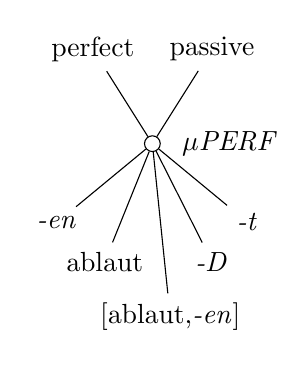
\begin{tikzpicture}[draw=black!100]
 	%[shorten >=1pt,->,draw=black!100]
	\def \rowatticone{4.0cm}
 	\def \rowtwoht{3.5cm}
	\def \rowtwohta{3.2cm}
 	\def \rowoneht{2cm}
	\def \rowzerohta{0.8cm}
	\def \rowzeroht{0.5cm}
	\def \basementone{0.0cm}
 	\tikzstyle{ms-node}=[text centered]
 	\tikzstyle{m-node}=[circle,draw=black!100,thin,inner sep=0pt,minimum size=2mm]
	\tikzstyle{pf-node}=[text centered]
 	\tikzstyle{m-lbl}=[text width=5ex]
	\node[m-lbl] (label0) at (13ex,\rowoneht) {$\mu{\textit{PERF}}$};
	
 	% morphosyntax
 	\node[ms-node] 	(ms0)	at (3ex,\rowtwohta)		{perfect};
 	\node[ms-node] 	(ms1)	at (13ex,\rowtwohta)	{passive};
	
 	% morphome
 	\node[m-node] 	(m0)	at (8ex,\rowoneht)		{};
	
	%phonological form
	 \node[pf-node] 	(pf0)	at (0ex,1cm)		{\textit{-en}};
 	\node[pf-node]  	(pf1)	at (4ex,\rowzeroht)		{ablaut};
 	\node[pf-node]  	(pf2)	at (9.5ex,-0.2cm)	 	{[ablaut,\textit{-en}]};
 	\node[pf-node]  	(pf3)	at (13ex,\rowzeroht) 		{\textit{-D}};
 	\node[pf-node] 	(pf4)	at (16ex,1cm) 		{\textit{-t}};	
	
 	\path (pf0)	edge	node	{}	(m0)
 		(pf1)	edge	node	{}	(m0)
 		(pf2)	edge	node	{}	(m0)
 		(pf3)	edge	node	{}	(m0)
		(pf4)	edge	node	{}	(m0)
		(m0) edge node 	{}	(ms0)
		(m0) edge node 	{}	(ms1);
		%(label0) edge node {}      (m0);	
 \end{tikzpicture}
\label{fig:ppgraph}
\caption{The English perfect participle: a polyvalent polymorphous metamorphome. The spokes radiating downward represent meromorphomes.}
\end{figure}

%\begin{figure}[ht]
%\centering
%%Monovalent monomorphous
%\subfigure[\label{fig:mtypes:mvmm}]{
%     \begin{tikzpicture}[draw=black!100]
% 	%[shorten >=1pt,->,draw=black!100]
%	\def \rowatticone{4.0cm}
% 	\def \rowtwoht{3.5cm}
%	\def \rowtwohta{3.2cm}
% 	\def \rowoneht{2cm}
%	\def \rowzerohta{0.8cm}
%	\def \rowzeroht{0.5cm}
%	\def \basementone{0.0cm}
% 	\tikzstyle{ms-node}=[text centered]
% 	\tikzstyle{m-node}=[circle,draw=black!100,thin,inner sep=0pt,minimum size=2mm]
%	\tikzstyle{pf-node}=[text centered]
% 	\tikzstyle{m-lbl}=[text centered]
%	\node[m-lbl] (morphome-label) at (5ex,\rowoneht) {$\mu{\textit{MENT}}$};
% 	% morphosyntax
% 	\node[ms-node] 	(ms0)	at (0ex,\rowtwoht)		{+noun};
% 	% morphome
% 	\node[m-node] 	(m0)	at (0ex,\rowoneht)		{};
%	%phonological form
%	 \node[pf-node] 	(pf0)	at (0ex,\rowzeroht)		{\textit{-ment}};
%
% 	\path (pf0)	edge	node	{}	(m0)
%		(m0) edge node 	{}	(ms0);		
% \end{tikzpicture}
%} %Monovalent polymorphous
%\subfigure[\label{fig:mtypes:mvpm}]{
%     \begin{tikzpicture}[draw=black!100]
% 	%[shorten >=1pt,->,draw=black!100]
%	\def \rowatticone{4.0cm}
% 	\def \rowtwoht{3.6cm}
%	\def \rowtwohta{3.2cm}
% 	\def \rowoneht{2cm}
%	\def \rowzerohta{0.8cm}
%	\def \rowzeroht{0.4cm}
%	\def \basementone{0.0cm}
% 	\tikzstyle{ms-node}=[text centered]
% 	\tikzstyle{m-node}=[circle,draw=black!100,thin,inner sep=0pt,minimum size=2mm]
%	\tikzstyle{pf-node}=[text centered]
% 	\tikzstyle{m-lbl}=[text centered]
%	\node[m-lbl] (morphome-label) at (12ex,\rowoneht) {$\mu{\textit{PAST}}$};
%	
% 	% morphosyntax
% 	\node[ms-node] 	(ms0)	at (7.5ex,3.0cm)		{past};
%	
% 	% morphome
% 	\node[m-node] 	(m0)	at (7.5ex,\rowoneht)		{}; %{$\mu{\textit{EN}}$};
%	
%	%phonological form
%	 \node[pf-node] 	(pf0)	at (0ex,\rowzerohta)		{$\emptyset$};
% 	\node[pf-node]  	(pf1)	at (3ex,\rowzeroht)		{\textit{-t}};
% 	\node[pf-node]  	(pf2)	at (7.5ex,\basementone)	 	{ablaut};
% 	\node[pf-node]  	(pf3)	at (12ex,\rowzeroht) 		{\textit{-d}};
% 	\node[pf-node] 	(pf4)	at (15ex,\rowzerohta) 		{\dots};	
%	
% 	\path (pf0)	edge	node	{}	(m0)
% 		(pf1)	edge	node	{}	(m0)
% 		(pf2)	edge	node	{}	(m0)
% 		(pf3)	edge	node	{}	(m0)
%		(pf4)	edge	node	{}	(m0)
%		(m0) edge node 	{}	(ms0);	
% \end{tikzpicture}
%}
%%Polyvalent polymorphous
%\subfigure[\label{fig:mtypes:pvpm}]{
%	\vspace{12pt}
%     \begin{tikzpicture}[draw=black!100]
% 	%[shorten >=1pt,->,draw=black!100]
%	\def \rowatticone{4.0cm}
% 	\def \rowtwoht{3.5cm}
%	\def \rowtwohta{3.2cm}
% 	\def \rowoneht{2cm}
%	\def \rowzerohta{0.8cm}
%	\def \rowzeroht{0.5cm}
%	\def \basementone{0.0cm}
% 	\tikzstyle{ms-node}=[text centered]
% 	\tikzstyle{m-node}=[circle,draw=black!100,thin,inner sep=0pt,minimum size=2mm]
%	\tikzstyle{pf-node}=[text centered]
% 	\tikzstyle{m-lbl}=[text width=5ex]
%	\node[m-lbl] (label0) at (13ex,\rowoneht) {$\mu{\textit{EN}}$};
%	
% 	% morphosyntax
% 	\node[ms-node] 	(ms0)	at (3ex,\rowtwohta)		{perfect};
% 	\node[ms-node] 	(ms1)	at (13ex,\rowtwohta)	{passive};
%	
% 	% morphome
% 	\node[m-node] 	(m0)	at (8ex,\rowoneht)		{};
%	
%	%phonological form
%	 \node[pf-node] 	(pf0)	at (0ex,1cm)		{\textit{-en}};
% 	\node[pf-node]  	(pf1)	at (4ex,\rowzeroht)		{ablaut};
% 	\node[pf-node]  	(pf2)	at (9.5ex,-0.2cm)	 	{[ablaut,\textit{-en}]};
% 	\node[pf-node]  	(pf3)	at (13ex,\rowzeroht) 		{\textit{-D}};
% 	\node[pf-node] 	(pf4)	at (16ex,1cm) 		{\textit{-t}};	
%	
% 	\path (pf0)	edge	node	{}	(m0)
% 		(pf1)	edge	node	{}	(m0)
% 		(pf2)	edge	node	{}	(m0)
% 		(pf3)	edge	node	{}	(m0)
%		(pf4)	edge	node	{}	(m0)
%		(m0) edge node 	{}	(ms0)
%		(m0) edge node 	{}	(ms1);
%		%(label0) edge node {}      (m0);	
% \end{tikzpicture}
% }
%% Polyvalent monomorphous
%\subfigure[\label{fig:mtypes:pvmm}]{
%     \begin{tikzpicture}[draw=black!100]
%	\def \rowatticone{4.0cm}
% 	\def \rowtwoht{3.5cm}
%	\def \rowtwohta{3.2cm}
% 	\def \rowoneht{2cm}
%	\def \rowzerohta{0.8cm}
%	\def \rowzeroht{0.5cm}
%	\def \basementone{0.0cm}
% 	\tikzstyle{ms-node}=[text centered]
% 	\tikzstyle{m-node}=[circle,draw=black!100,thin,inner sep=0pt,minimum size=2mm]
%	\tikzstyle{pf-node}=[text width=12ex, text centered]
% 	\tikzstyle{m-lbl}=[text width=5ex]
%	\node[m-lbl] (label) at (11ex,1.5cm) {$\mu{Z}$};
%	
% 	% morphosyntax
%	 \node[ms-node] 	(ms0)	at (0ex,2.5cm)			{clitic};
% 	\node[ms-node]  	(ms1)	at (4ex,3.2cm)		{poss.};
% 	\node[ms-node]  	(ms2)	at (9 ex,3.2cm)	 	{n.pl};
% 	\node[ms-node]  	(ms3)	at (13ex,2.5cm) 		{v.3sg};
% 	% morphome
% 	\node[m-node] 	(m0)	at (6ex,1.5cm)		{};
%	
%	%phonological form
% 	\node[pf-node]  	(pf0)	at (6ex,0.0cm)	 	{\textit{-Z}};
%
% 	\path (pf0)	edge	node	{}	(m0)
% 		(m0)	edge	node	{}	(ms0)
% 		(m0)	edge	node	{}	(ms1)
% 		(m0)	edge	node	{}	(ms2)
%		(m0)	edge	node	{}	(ms3);
%		%(label)  edge  node {}     (m0);		
% \end{tikzpicture}
%}
%\caption[]{Round's is not the only morphome taxonomy. \cite{aronoff:md:2016} classifies morphomes by complexity. 
%Subfigure \subref{fig:mtypes:mvmm} represents the  
%\textbf{monovalent monomorphous} type, 
%\subref{fig:mtypes:mvpm} the \textbf{monovalent polymorphous} type, 
%\subref{fig:mtypes:pvpm} the \textbf{polyvalent polymorphous} type, 
%and \subref{fig:mtypes:pvmm} the \textbf{polyvalent monomorphous} type. (This 
%diagram is a reproduction of the one in \cite{aronoff:md:2016}.) } 
%\label{fig:mtypes}
%\end{figure}

\paragraph{Meromorphomes.} Whereas rhizomorphomes and metamorphomes 
transcend the realms of individual lexemes and paradigms and thus highly 
abstract, meromorphomes are comparatively concrete, as they 
correspond to particular parts of word forms. Meromorphomes, it must be said, 
are not the word parts themselves, since all morphomes reside at the 
morphomic level rather than the phonological, or surface, level \citep{round:2011}. 
Even so, meromorphomes map directly onto phonological forms, and 
are thus more closely associated with phonological forms than rhizomorphomes 
or metamorphomes. Indeed, both rhizomorphomes and metamorphomes are 
composed of meromorphomes, since, at some point, the abstract, trans-lexemic 
types of morphomes must interact with specific phonological forms. 

For instance, in English perfect participles, each individual root, e.g., \textit{s-ng}, 
\textit{br-k}, \textit{kick}, etc., is a meromorphome. Each suffix 
as well as each particular variety of ablaut is also a meromorphome. 
The Romance L-morphome is also composed of particular meromorphomes. 
Within the paradigm of the lexeme \textsc{decir} \textsc{`to say'} 
(table \ref{tab:l-morphome}). The stem \textit{dig-} is a meromorphome. 
Similarly, the stem \textit{crezc-} is a meromorphome within the paradigm of 
\textsc{crecir} \textsc{`to grow'}. %Each distinct stem (which vary across paradigms)
%correspond to``concrete" pieces of form. They are the raw material from which paradigms are constructed. 

\begin{table}[ht]
\begin{center}
\subtable[maqomi `local' \label{subtab:fusion:1}]{
{\begin{tabular}{lcc}
\  & masc & fem  \\
\hline 
sg & maqom-i & meqom-i-t  \\
pl & meqom-iy-im & meqom-iy-ot  \\
\end{tabular}}
}
\subtable[gadol `big' \label{subtab:fusion:2}]{
{\begin{tabular}{lcc}
\  & masc & fem  \\
\hline 
sg & gadol & gdol-a  \\
pl & gdol-im & gdol-ot  \\
\end{tabular}}
}
\label{tab:fusion}
\caption{Fusional suffixes in Hebrew nominals}
\end{center}
\end{table}

\subsection{An example from Hebrew}
\label{sec:heb-example}
We turn now to a case of syncretism in the morphology of Modern Hebrew. Perhaps
the best known aspect of Hebrew (and Semitic languages in general) is its 
non-concatenative root-and-pattern morphology. But 
Hebrew's morphology also has a rich concatenative component, consisting of
of both inflectional and derivational affixes. Moreover, the inflectional affixes tend to be
highly (and idiosyncratically) fusional.  
Consider the forms in table~\ref{tab:fusion}. 

In this section, we shall primarily be concerned with the
interaction between \textit{-t} and \textit{-i} in Hebrew feminine endings.
Hebrew uses the vowel [i] 
as a suffix both to derive adjectives and to derive nouns.
As illustrated in table~\ref{subtab:der-adjectives}, 
one can derive adjectives 
in Hebrew by attaching \textit{-i} to noun bases. The \textit{-i} 
must be the `adjective' exponent
in table \ref{subtab:der-adjectives} because it is the only suffixal 
element to occur in each
of the four columns. % It must therefore be the adjectival exponent in these cases. 
\begin{table}[ht]
   \centering
   \caption{Derivational and inflectional syncretism in Hebrew feminine endings.}\label{tab:deriv} 
   \subtable[Adjectives derived from nouns via \textit{-i}\label{subtab:der-adjectives}]{
     \centering
        \begin{tabular}{l l l l c}
       \toprule
        \textsc{noun base} &  \textsc{masc.sg} & \textsc{fem.sg} &  \textsc{fem.pl} & \textsc{gloss} \\ %[0.5ex]
        \midrule
        %tarbut \textit{`culture'} & tarbut-i & tartbut-i-t & tarbut-iy-ot & `cultured' \\
        %le\textipa{P}om \textit{`nation'} & le\textipa{P}omi & le\textipa{P}omit & le\textipa{P}omiyot  & `national' \\
        merxav \textit{`space'} & merxav-i  &  merxav-i-t  &  merxav-iy-ot   &  `spatial' \\
        \textipa{P}aviv \textit{`spring'} & \textipa{P}aviv-i & \textipa{P}aviv-i-t & \textipa{P}aviv-iy-ot  & `spring-like' \\
        \textipa{P}arec \textit{`land'} & \textipa{P}arc-i & \textipa{P}arc-i-t & \textipa{P}arc-iy-ot  & `earthly' \\
        \bottomrule 
    \end{tabular}
   }\\
\vspace{6pt}
      \subtable[Nouns derived via \textit{-it}\label{subtab:der-nouns-i}]{
     \centering
    \begin{tabular}{l l l c} % creating 3 columns
   \toprule
    \textsc{base} &  \textsc{sg} &  \textsc{pl} & Gloss \\ 
    \midrule
    %pax \textit{`tin'} & pax-it & pax-iy-ot & `tin can' \\
    ma\d{s}a\textipa{P} `cargo' & ma\d{s}a\textipa{P}-it  &   ma\d{s}a\textipa{P}-iy-ot  &   `truck'   \\
    xalal \textit{`space'} & xalal-it & xalal-iy-ot & `spaceship' \\
    %k.r.k \textit{`(to) wrap'} &  kru\d{k}-it   &   kru\d{k}iy-ot  & `strudel' \\ %(iff \textit{fem}) or \\
    nagar \textit{`carpenter'}  &  nagar-it   &   nagr-iy-ot  & `female carpenter' \\
    \bottomrule
    \end{tabular}
   }\\
   \vspace{6pt}
   \subtable[Nouns derived via \textit{-ut}\label{subtab:der-nouns-u}]{
     \centering
        \begin{tabular}{l l l c}
        \toprule
        \textsc{base} &  \textsc{sg} &  \textsc{pl} & \textsc{gloss} \\ %[0.5ex]
        \midrule
        ma\v{s}ma\textrevglotstop \textit{`meaning'} & ma\v{s}ma\textrevglotstop-{u}t & ma\v{s}ma\textrevglotstop-{u}y-ot & `importance' \\
	\v{s}agrir \textit{`ambassador'} & \v{s}agrir-ut & \v{s}agriruy-ot & `embassy' \\
        %b.g.r \textit{`(to) mature'}  &  bagr-ut  &  bagr-uy-ot  &  `matriculation exam' \\
        nagar \textit{`carpenter'} &  nagar-ut   &   nagr-uy-ot  & `carpentry' \\
        \bottomrule
	\end{tabular}
   }
%\caption{Subtable (\ref{subtab:der-adjectives}) presents several adjectives 
%that are derived from nouns via the %adjective-deriving 
%\textit{-i} suffix. 
%Feminine adjectives are formed by attaching \textit{-t} to the \textit{-i} of the masc. form. Subtable 
%(\ref{subtab:der-nouns-i}) shows a different suffixal function of \textit{-i}, but here it is used 
%in conjunction with \textit{-t} to derive nouns instead of adjectives. Finally, 
%subfigure (\ref{subtab:der-nouns-u}) illustrate another nominalization suffix, 
%namely \text{-u.}}
%Realizations of the morphomes $\mu$\textsc{i}, $\mu$\textsc{t}, $\mu$\textsc{o}, and $\mu$\textsc{u} in the suffixes
%\textit{-i(t)}, \textit{-it}, \textit{-ot}, and \text{-ut}.}
\end{table}
Thus, \textit{merxav} `space' + \textit{-i} = \textit{merxav-i} 
`spatial (masc.sg)'. The fem.sg is obtained by attaching \textit{-t} to the masc.sg
form. Feminine adjectives thus end in \textit{-it}. 
Hebrew also uses \textit{-it} to derive nouns, usually by attaching it 
to nouns, as in in table~\ref{subtab:der-nouns-i}. 
The vast majority of nouns derived in this way are feminine in 
grammar, semantics, or both. 


%When used to
%derive nouns, \, i.e., feminine , usually from 
%other nouns, by attaching the suffix \textit{-it} to the base, 
%as in table \ref{subfig:der-nouns-i}. 

%However, the ending \textit{-it} also occurs
%in the derived adjectives subtable, but in this case
%it is composed of two suffix. %It is evident that 
%The \textit{-i} is the common adjective-deriving 
%unit across the table's columns, since it is the 
%difference between each base base and 
%its corresponding form in the \textit{masc.sg} adjective 
%column  (e.g., \textit{merxav} `space' ~ \textit{merxav-i} 
%`spatial')

%\begin{table}[h]
%\centering % centering table
%\begin{tabular}{c c c c c c} % creating 3 columns
%\hline\hline %inserting double-line
%Lexical cat. & Lexeme &\textsc{m.sg} & \textsc{f.sg} &  \textsc{m.pl} & \textsc{f.pl}\\ [0.5ex]
%\hline % inserts single-line
%Adjectives & \textsc{local} & maq\'om &   maqom\'i   &  mqom\'it   &   mqomiyi\'ot \\
%	&	& maqom & maqom+$\mu${\textsc{adj}} & maqom+$\mu${\textsc{adj}}+$\mu${\textsc{t}} & maqom+$\mu${\textsc{adj}}+$\langle \mu${\textsc{o}}-$\mu$\textsc{t} $\rangle$ \\
%	&	& \textsc{maqom} & \textsc{maqom}+\textsc{adj}+\textsc{m.pl} & \textsc{maqom}+\textsc{adj}+\textsc{f.sg}  & \textsc{maqom}+\textsc{adj}+\textsc{f.pl} \\
%Participles & \textsc{tell} & mesap\'er & mesapr\'im  & mesap\'eret &  mesapr\'ot\\
%	&	& mesaper & mesaper+$\mu${\textsc{adj}} & mesaper+$\mu${\textsc{adj}}+$\mu${\textsc{t}} & mesaper+$\mu${\textsc{adj}}+$\langle \mu${\textsc{o}}-$\mu$\textsc{t} $\rangle$ \\
%	&	& \textsc{mesaper} & \textsc{s.p.r}+\textsc{adj}+\textsc{m.pl} & \textsc{mesaper}+\textsc{adj}+\textsc{f.sg}  & \textsc{mesaper}+\textsc{adj}+\textsc{f.pl} \\
%\hline % inserts single-line
%\end{tabular}
%\label{tab:hresult}
%\caption{Performance Using Hard Decision Detection} %title of the table
%\end{table}

%\begin{figure}[h]
%\begin{center}
%\subfigure[Adjectives derived via +\textit{i}\label{subfig:der-adjs-i}]{
%\begin{tabular}{c c c c c c} % creating 3 columns
%%\centering % centering table
%%\caption{Derived Adjectives.}\label{tab:hresult}
%\toprule%inserting double-line
%\textsc{noun base} &  \textsc{masc.sg} & \textsc{fem.sg} &  \textsc{fem.pl} & Gloss \\ [0.5ex]
%\midrule
%tarbut (`culture') & tarbuti & tartbutit & tarbutiyot & `cultured' \\
%le\textipa{P}om (`nation') & le\textipa{P}omi & le\textipa{P}omit & le\textipa{P}omiyot  & `national' \\
%merxav (`space') & merxavi & merxavit & merxaviyot  & `spatial' \\
%\textipa{P}aviv (`spring') & \textipa{P}aviv i & \textipa{P}aviv it & \textipa{P}aviviyot  & `spring-like' \\
%le\textipa{P}arec (`land') & le\textipa{P}arci & le\textipa{P}arcit & le\textipa{P}arciyot  & `earthly' \\
%\bottomrule % inserts single-line
%%\label{subfig:der-adjs-i}
%\end{tabular}
%} \\
%\subfigure[Nouns derived via \label{subfig:der-nouns-i}]{ %+\textit{i}]{
%\begin{tabular}{c c c c} % creating 3 columns
%\hline
%\textsc{base} &  \textsc{sg} &  \textsc{pl} & Gloss \\ [0.5ex]
%\hline
%pax (`tin') & paxit & paxiyot & `cultured' \\
%ma\d{s}a\textipa{P} (`load') & ma\d{s}a\textipa{P}it  &   ma\d{s}a\textipa{P}iyot  &   `truck'   \\
%$\sqrt{\text{k.r.k}}$ (`bind, wrap')  &  kru\d{k}it   &   kru\d{k}iyot  & `strudel' (iff \textit{fem}) or `@' (iff \textit{masc}) \\
%nagar (`carpenter')  &  nagarit   &   nagriyot  & `female carpenter'
%\hline % inserts single-line
%%\label{subfig:der-nouns-i}
%\end{tabular}
%}  
%\subfigure[Nouns derived via +\textit{u}\label{subfig:der-nouns-u}]{
%\begin{tabular}{c c c c}
%\textsc{base} &  \textsc{sg} &  \textsc{pl} & Gloss \\ [0.5ex]
%\midrule
%\v{s}agrir (`ambassador') & \v{s}agrirut & \v{s}agriruyot & `embassy' \\
%$\sqrt{\text{b.g.r}}$  (`mature') &  bagrut & bagruyot &  `matriculation exam' \\
%nagar (`carpenter')  &  nagarut   &   nagruyot  & `carpentry'
%\bottomrule %maiden:2005 inserts single-line
%%\label{subfig:der-nouns-u}
%\end{tabular}
%} 
%\end{center}
%\caption{The \textit{t} quasi-morpheme}
%\label{fig:t}
%\end{figure}
In Hebrew, feminine words frequently 
end in \textit{-t}. Indeed, the co-occurrence of \textit{-t} and the feminine gender is 
too frequent to be the product of random chance \citep{faust:2013}.
In fact, \textit{-t} serves as an exponent of both grammatical (or \emph{inflectional}) 
gender as well as semantic (or \emph{derivational}) gender. For example, /-t/ 
is an inflectional ending in \textit{merxavit} `spatial (fem.)' 
(cf. the corresponding masc. form \textit{merxavi}). 
It is as part of the derivational suffix \textit{-it}, used to 
derive semantically feminine nouns, in \textit{nagar-it} 
`female carpenter' (cf. \textit{nagar}`(male) carpenter'). 
Tables~\ref{subtab:der-adjectives} and \ref{subtab:der-nouns-i} 
show additional
examples of these two disparate functions of \textit{-i}.

\subsection{A morpheme-based approach}
The ending \textit{-t}, when used as (part of) a suffix on 
nominal forms, is always accompanied by a vowel. 
In fact, it appears with each of Modern Hebrew's five vowels.
In singular-form endings, it appears with every vowel except 
\textit{o}: \textit{-at}, \textit{-(e)t}, \textit{-ut}, and \textit{-it}. 
It appears with \textit{o} in the feminine plural suffix \textit{-ot} 
also ends with \textit{t}. \footnote{The consonant /t/ occurs with 
/o/ in singular forms as well, but only when /-ot/ is part of a 
primitive word, as in, e.g., \textipa{P}ot `letter'.}

Besides \textit{-t}, the only other systematic feminine marker is 
\textit{-a}, which is found only 
in fem.sg absolute-state forms. [Examples]
But a final \textit{-t} appears even in these nouns when they are 
in the construct state, a type of form which is used compound-noun 
construction and marked by its complete lack of stress.
\cite{schwarzwald:1982} argues that
the construct-state's \textit{t} ending was once also 
present on the absolute \textit{-a}, but was lost through a historical
\textit{t-}deletion process. \cite{faust:2013}, however, 
goes a step further, arguing that the \textit{t} remains 
underlyingly present in \textit{-a} even today. According 
to \cite{faust:2013}, both
\textit{-a} and \textit{-t} are underlyingly /-at/; sometimes 
the \textit{a} deletes, and sometimes the \textit{-t} deletes, depending 
upon certain phonological factors. Sometimes they appear 
together in the same form, as in fem.sg construct nouns
Faust additionally decomposes the derivational endings 
\textit{-ut} and \textit{-it} into /u-at/ and /i-at/, respectively. 
The \textit{a} deletes in these forms.
%\cite{faust:2013} thus analyzes the \textit{t} as the universal feminine morpheme of Hebrew\footnote{Faust
%takes an approach based on Distributed Morphology (DB) \cite{halle-and-marantz:1993}, a \emph{morpheme}-based 
%approach.}. Faust moreover decomposes the suffixes \textit{-it}, and \textit{-ut} each into
%two morphemes: the feminine /t/ and /i/, and /u/, respectively. (
%(The suffixes \textit{-et} in \textit{-at} are  regarded 
%by Faust as allophonic.) 
Faust regards \textit{-et} in \textit{-at} as both allophones of /-at/. 
Faust's analysis of the Hebrew feminine endings thus constitutes a total of 
four morphemes, namely /-i/, /-u/, /-at/, and /-o/.

%In the remainder of this discussion, we shall be primarily concerned with /i/, which particularly interesting because
%there seem to be two distinct morphological units /i/.

%\cite{faust:2013} analyzes the Modern Hebrew feminine 
%%In any case, he latter was lost 
%%``through a process of final \textit{t}deletion in absolute state forms" (p. 159). 
%that the current that the modern \textit{-a} ending 
%absolute \cite{schwarzwald:1982, faust:2013} lists the following as the set 
%of possible feminine endings in 
%
%Faust argues that the suffix \textit{-at} is a \emph{root} is such that it selects for another root as its complement. 
%That is, it will only attach to another morpheme of root status
 

%Faust argues that the suffix \textit{-at} is such that it selects for another root as its complement. That is, it will only attach to another morpheme of root status. Note that root here is the technical term of Distributed Morphology \cite{}, not necessarily the consonantal root of Semitic languages, although consonantal roots would certainly be a subset of \ac{DM} roots. 
  
   \begin{table}
     \centering
%        \begin{tabular}{l l c }
%       \toprule
%        \textsc{Morphome} &  Phon. & \\ [0.5ex]
%        \midrule
%       \textsc{fem} & $\mu{\textsc{a}}$ & $\Phi_{\text{A}}$ & {/\'a/, /-at/} \\
%       \textsc{base}$\to${adj}, \textsc{base}$\to$\textsc{noun} &$\mu{\textsc{i}}$ & $\Phi_{\textsc{i}}$ & {/+i/, /+it/} \\
%       $\mu{\textsc{a}}$ & $\mu{\textsc{u}}$ & $\Phi_{\text{U}}$  & {/-ut/} \\
%       $\mu{\textsc{a}}$ & $\mu{\textsc{o}}$ & $\Phi_{\text{O}}$ & {/-ot/}  \\
%       $\mu{\textsc{a}}$ & $\mu{\textsc{t}}$ & $\Phi_{\text{T}}$ & {/-ot/, /-t/} \\
%        \bottomrule 
%    \end{tabular}
       \begin{tabular}{c c c }
       \toprule
        \textsc{Morphome} &  Phon. suffixe(s) & Morphosyntactic property set(s) \\ [0.5ex]
        \midrule
       $\mu{\textsc{a}}$ & {/-\textbf{a}/},{/-\textbf{a}t/} & \{fem, sg,\textsc{state:}abs\}, \{fem, sg, \textsc{state:}constr\}\\
       $\mu{\textsc{i}}$ & {/-\textbf{i}/, /-\textbf{i}t/} & \text{n}$\to${adj}, \text{n}$\to$\text{n}[fem] \\
       $\mu{\textsc{u}}$ & {/-\textbf{u}t/} & \text{n}$\to$\text{n}[fem, -concrete] \\
       $\mu{\textsc{o}}$ & {/-\textbf{o}t/} & \{fem, pl\} \\
       $\mu{\textsc{t}}$ & { /-\textbf{t}/, /-o\textbf{t}/, /-u\textbf{t}/, /-i\textbf{t}/}  & \{fem\}, \{fem, pl\}, \{fem, -concrete\}, \\
        \bottomrule 
    \end{tabular}
    \caption{Morphomic and Phonological Operations}
    \label{tab:heb-morphomes}
    \end{table}
    
Faust's approach is based on Distributional Morphology 
 \citep{halle-and-marantz:1993}, 
a morpheme-based, Lexical-Realizational theory \citep{stump:2001}
According to Faust, therefore, the suffixes /-i/, /-u/, and /-at/ are not only morphemes, 
but \emph{roots.}
In \ac{DM}, the term \emph{root} (along with \emph{formative}) is used to refer 
to maximally primitive units of meaning. (It is not to be confused with the 
consonantal root of Semitic morphology. Semitic roots would qualify as 
\ac{DM} roots, but the \ac{DM} root is more general than the Semitic root.)
A \ac{DM} root has no particular morpho properties and thus belongs to 
no morphosyntactic category.
However, it does have abstract semantic features as well as inherent 
selectional requirements, i.e., criteria that limit the set of stems with which it 
may combine. In particular, roots exclusively select 
other roots as their complements. %That is to say, roots combine only with roots.  

Because \textit{-at} is a root, therefore, it
never attaches to derived stems. The same is true of /-i/ and /-u/.  
However, \textit{-at} is distinguished from /-i/ and /-u/ in that it occupies the 
position of category head in the derivation of adjectives.
Of course, the suffix /-at/ is not present in the derivations of 
masculine adjectives, 
but the position of category head is. 
It is just phonologically null, according to \ac{DM}.
In such cases, the suffix /-i/ simply combines with the null adjectival head. 
This, according to Faust, satisfies the selectional requirements of /-i/
and the null adjectival head. The rest of the derivation,
proceeds as it does in feminine adjectives. 

%is a root that will attach only to another root. Faust argues that it never attaches to bases that are derived words or loanwords. (The latter, Faust supposes, have a derived status by virtue of the borrowing process. By contrast, -i- and -u- frequently combine with non-roots. 
According to Faust, \textit{-at} sometimes uses \textit{-i} and 
\textit{-u} as buffers. That is, it first attaches to \textit{-i} or \textit{-u}, 
thus forming complex units, either \emph{-it} or \emph{-ut}, respectively, 
which then attach to
the non-primitive stem. Because \emph{-it} and \emph{-ut} are complex, 
they cannot be roots and are thus free of roots' selectional constraints.

%That is, they first attach to
%-i- or -u-, thus forming -it or -ut (the a is deleted), which can then attach to any base, including all manner of derived bases. 

Moreover, Faust argues that the adjectival \textit{-i} and 
the noun-deriving \textit{-i} ending in tables 
\ref{subtab:der-adjectives} and \ref{subtab:der-nouns-i} 
are in fact one and the same expletive morpheme. That is, 
/-i/ does not per se mean `\textsc{adjective}' in the derived adjectives 
\ref{subtab:der-adjectives}. It is rather an expletive suffix, one that 
crucially, for Faust, lacks morphosyntactic properties.
%The seemingly noun-deriving
%suffix \textit{-i} is, according to Faust, the same expletive root. 
Note that it is \ac{DM} that motivates Faust's decision to posit a single 
expletive /-i/ morpheme (as opposed to 
separate adjective-deriving and noun-deriving morphemes).  Faust 
requires /-i/ to be a \ac{DM} root so that /-at/ can combine with it, and since 
\ac{DM} roots must be free of any specification of morphosyntactic 
category, an intrinsically adjectival /-i/ would
not suit Faust's \ac{DM} analysis. 

%If /-i/
%If there were an (intrinsically) adjective-deriving /-i/, it would occupy 
%the position of adjectival head within the word-internal syntax
%and thus could not be a \ac{DM} root.  
%Note also that a more conventional 
%morpheme-based analysis would likely conclude that there are 
%two separate morphemes 
%here, namely two /-i/ suffixes that are identical 
%in form, but distinct in meaning. 


\subsection{A \emph{morphome}-based approach}
As it turns out, Faust's account and a \emph{morphome}-based approach 
are similar top each other in at least one respect, namely in the analysis of /-i/
as a single (unified) morphological unit. But whereas Faust posits a unified 
/-i/ morpheme, we shall posit here a 
a unified \emph{morphome} $\mu{\textsc{i}}$. Like Faust's expletive /-i/,
%However, from a morphome-based perspective, this is a morphome (or more 
%precisely the phonological manifestation
%of /-i/'s morphomic representation.) 
$\mu{\textsc{i}}$ has no meaning in and of itself, but this is not 
because $\mu{\textsc{i}}$ is entirely unassociated with meaning; 
$\mu{\textsc{i}}$ lacks intrinsic meaning because meaning is not the 
purview of a morphomic representation. Rather, meaning is supplied by 
the lexical level. One of the advantages of a morphomic approach
is that any number of different meanings can be mapped onto a single 
morphome. We shall also posit a morphome corresponding to the 
feminine ending \textit{-a} and a \emph{different} morphome for 
\textit{-t}, as there does not seem to be enough synchronic evidence to posit that 
\textit{-a} and \text{-t} both have the \emph{synchronic} 
underlying form /-at/.
 \begin{figure}[ht]
  \small
\begin{center}
   \subfigure[{\textglotstop}{avavit} `spring-like'\label{subtab:heb-avivit}]{
     \centering
        \begin{tabular}{l c c c}
       \toprule
        \multicolumn{4}{c}{[\textipa{P}avivit] `spring-like'}\\
        \midrule
        \multirow{2}{*}{Phonological} & \textipa{P}aviv & -i & -t \\ %\hline
         %& $\Phi{\textsc{stem}} (\text{a.i}, \text{\textipa{P}.b.b} )$ & $\Phi_{\textsc{i}}$ & $\Phi_{\textsc{t}}$ \\ %\hline
         %& $\Phi{\textsc{stem}} (\text{a.i}, \textsc{\textipa{P}bb})$ & $\Phi{\textsc{i}}$ & $\Phi{\textsc{t}}$ \\
         & $\Phi${\textsc{stem}} & $\Phi${\textsc{i}} & $\Phi${\textsc{t}} \\
       Morphomic & $\mu$\textsc{a-i}, $\surd \textsc{\textipa{P}-b-b}$ & $\mu{\textsc{i}}$  & $\mu{\textsc{t}}$ \\ 
        Lexical & \multicolumn{3}{c}{$\surd \textsc{\textipa{P}-b-b}$, \{\text{adj}, \text{fem}, \text{sg}\}}\\
        \bottomrule 
    \end{tabular}
    }
%      \vspace{7pt}
%   \subtable[xalalit `spaceship'\label{subtab:heb-xalalit}]{
%     \centering
%        \begin{tabular}{l r}
%       \toprule
%        \multicolumn{2}{c}{xalalit}\\
%        \midrule
%        \multirow{2}{*}{Phonological} & xalal-it \\ %\hline
%         %& $\Phi_{\textsc{stem}}$ %( \textipa{a.a}, \text{\textipa{x.l.l}} )$ 
%        & $\Phi{\textsc{it}}$, $\Phi_{\textsc{stem}}$ \\ %\hline
%        Morphomic & $\mu{\textsc{t}}$, $\mu{\textsc{i}}$, $\mu{\textsc{\textipa{a.a}}}$, $\surd \text{xll}$\\ %\hline
%        Lexical & $\surd \textsc{xll}$, \{\text{noun}, \text{fem}, \text{sg}\} \\
%        \bottomrule 
%    \end{tabular}
%    }
    \vspace{6pt}
      \subfigure[xalalit\label{subtab:heb-xalalit}]{
     \centering
    \begin{tabular}{l c c}
       \toprule
          \multicolumn{3}{c}{[xalalit] `spaceship'}\\
        \midrule
          \multirow{2}{*}{Phonological} & xalal & -it \\
           & $\Phi$\textsc{stem} & $\Phi$\textsc{it} \\
           Morphomic & $\mu$\textsc{a.a}, $\surd$\textsc{x-l-l} & $\mu$\textsc{i}, $\mu$\textsc{t} \\ 
            Lexical & \multicolumn{2}{c}{$\surd$\textsc{x-l-l}, \{\text{noun}, \text{fem}, \text{sg}\}}\\
       \bottomrule 
    \end{tabular}
    }
%      \vspace{7pt}
%  \subtable[\textglotstop{aviviyot}\label{subtab:heb-aviviyot}]{
%    \centering
%        \begin{tabular}{l c c c}
%       \toprule
%       % //\textsc{noun base} &  \textsc{masc.sg} & \textsc{fem.sg} \\ [0.5ex]
%        \multicolumn{5}{c}{\textipa{P}aviviyot `spring-like (\textsc{pl})}\\
%        \midrule
%        \multirow{2}{*}{Phonological} & \textipa{P}aviv & i & ot \\ %\hline
%         & $\Phi_{\textsc{stem}}$ 
%         %s( \text{a.i}, \text{\textipa{P}.b.b} )$ 
%         & $\Phi_{\textsc{i}}$ & $\Phi_{\textsc{ot}}$ \\ %\hline
%        Morphomic & $\mu{\text{a.i}}$, $\surd \text{\textipa{P}bb}$ & $\mu{\textsc{i}}$  & \multicolumn{2}{c}{$\mu{\textsc{o}}$, $\mu{\textsc{t}}$} \\ %\hline
%        Lexical & \multicolumn{4}{c}{$\surd \text{\textipa{P}bb}$, \{\textsc{+adj}, \textsc{+fem}, \textsc{+pl}\}}\\
%        %$\mu{\textsc{t}}$ & $\Phi_{\text{T}}$ & {/t/} \\
%        \bottomrule 
%    \end{tabular}
          \vspace{6pt}
  \subfigure[xalaliyot `spaceships'\label{subtab:heb-xalaliyot}]{
    \centering
        \begin{tabular}{l c c c }
       \toprule
       % //\textsc{noun base} &  \textsc{masc.sg} & \textsc{fem.sg} \\ [0.5ex]
        \multicolumn{4}{c}{[\textipa{x}alaliyot] `spaceships'}\\
        \midrule
        \multirow{2}{*}{Phonological} & xalal & i & ot \\ 
         & $\Phi$\textsc{stem}
         %s( \text{a.i}, \text{\textipa{P}.b.b} )$ 
         & $\Phi$\textsc{i} & $\Phi$\textsc{ot} \\ 
        Morphomic & $\mu${\textsc{a-a}}, $\surd$\textsc{x-l-l} & $\mu$\textsc{i}  &  $\mu$\textsc{o}, $\mu$\textsc{t} \\
                            %\multicolumn{2}{c}{$\mu$\textsc{o}, $\mu$\textsc{t}} \\ %\hline
        Lexical & \multicolumn{3}{c}{$\surd$\textsc{x-l-l}, \{\text{noun}, \text{fem}, \text{pl}\}}\\
        \bottomrule 
    \end{tabular}
  }
    \caption{\textit{Morphomic analyses.}  }
    \label{tab:heb-morphomic-analyses}
    \end{center}
    \end{figure}
% in the present day, nor does there seem to 
%be sufficient evidence to posit that \textit{-t} is underlyingly /-at/.
 Finally, we shall posit distinct morphomes for the abstract (-\textsc{concrete}) 
 nominalizing suffix \textit{-u}
 as well as the \textit{-o} in the feminine plural \textit{-ot}.
That is, following \cite{faust:2013}, we shall
decompose not only /-it/, but /-ut/ and /-ot/ as well. 
%the feminine plural \textit{-ot} into \textit{-o} 
%and \textit{-t}, each corresponding to a distinct morphome at the 
%morphomic level.

   
  Accordingly, we need a total of five morphomes
  to account Hebrew's range of feminine suffixes. These are presented in table \ref{tab:heb-morphomes}. 
  Note that the mapping from 
  morphomes to phonological suffixes is not one-to-one. For example, 
  $\mu{\textsc{i}}$ maps to the adjective-deriving suffix /-i/. It also 
  plays a part in the realization of the noun-deriving suffix /-it/. Now, 
  this noun-deriving /-it/ is a single \emph{non-decomposable} suffix at the phonological 
  level. The evidence for this is the fact that the /t/ cannot be detached 
  from the /i/ when /-it/ is serving a noun-deriving purpose. Consider, for 
  example, nagar-it `female carpenter', which is derived from the suffix-less, 
  masculine noun base \emph{nagar} `(male) carpenter'. 
There is no *\emph{nagar-i}.
  
Together, $\mu\textsc{i}$ and $\mu\textsc{t}$ form what is in effect  
a \emph{complex morphome} \citep{round:2015, round:md:2016}. A single 
phonological operation maps $\langle \mu\textsc{i}$, $\mu\textsc{t} \rangle$ 
onto a single morphological unit in the phonological output, namely the 
noun-deriving /-it/. The formation of the complex morphome $\langle \mu\textsc{i}$, 
$\mu\textsc{t} \rangle$ is conditioned upon presence of the 
property \{\text{n}$\to$\text{n}[fem] among the derivational properties $\delta$.
 
% The reason we want this pair 
% of morphomes to map to a monolithic phonological representation
% %important We want the nominalizing /-it/ to be represented at the phonological level as a single suffix because
%is that the /t/ cannot be detached from the /i/ when /it/ is serving the purpose 
%of noun-derivation; the noun-deriving /-it/ is always attached to a masculine noun base
%as a whole. Consider, for example nagar-it `female carpenter', which is derived from 
%the suffix-less, masculine noun base \emph{nagar} `(male) carpenter'. There is no 
% *\emph{nagar-i}.

  By contrast, consider the masc.sg adjective form \emph{\textglotstop{aviv-i}} 
  `spring-like', derived from the \emph{\textglotstop{aviv} `spring'}, 
  as well its feminine-adjective inflection  \emph{\textglotstop{aviv-i-t}}. Here, the /-t/ 
  is very much detachable; its removal simply produces the masculine form. We
  thus regard the feminine adjective ending as decomposable even at the 
  phonological level, and thus there can be no complex morphome $\langle \mu\textsc{i}$, 
  $\mu\textsc{t} \rangle$ at the morphomic level. The same morphomes are present in the 
  morphomic representation of \emph{\textglotstop{aviv-i-t}}, but they are each 
  independently mapped to phonological representations.
  
  It is important that the same morphomes be present in the morphomic 
  representations of both noun-deriving and adjectival instances of /-it/, 
  even if the mappings from morphomes to the phonological level are different. We 
  want to acknowledge that the identities of form are not accidental, 
  and that there is sameness here at some level. The purpose of the 
  morphomic level is to account for
  this sort of sameness.
  
 We shall analyze /-ot/, the fem.pl. suffix, and /-ut/, the abstract (or \textsc{concrete:}[-])
 noun-deriving suffix, in a similar way. Both are monolithic suffixes at the phonological
 level, and both have complex morphomic representations. Again, the primary reason for this
 is that neither /-ot/ nor /-ut/ seem to be decomposable, at least not in a straightforward
 way; that is, /-ot/ as a whole is the fem.pl suffix. If /-t/ is the fem. suffix, then
 /-o/ should be plural suffix. If this were the case, we would expect to see
 /-o/ in the masc.pl. ending, but the masc.pl. suffix is in fact /-im/. The suffix /-ot/
 corresponds to the morphome pair $\langle \mu\textsc{o}$, $\mu\textsc{t} \rangle$, 
 as shown in table \ref{subtab:heb-xalaliyot}, and /-ut/ to $\langle \mu\textsc{u}$, 
 $\mu\textsc{t} \rangle$. Analyzed in this way, /-ot/ and /-it/ share the morphome 
 $\mu$\textsc{t} with /-it/, thus accounting for the fact that all three suffixes end 
 in /-t/. The morphome $\mu\textsc{t}$ is thus used both derivationally and 
 inflectionally, a kind of dual appropriation that is not unknown among the world's languages. 
 Round, for instance, has frequently observed it in Kayardild: ``[M]ost of the exponents 
 employed by the inflectional system are also used derivationally" \citep[][p. 13]{round:2015}.
  
%that is, a morphomic representation separate from both
%the lexical and the phonological levels. We thus allow it to
%be associated with two separate meanings at once. 

%In Hebrew, all category heads are roots, and a root will not combine with a 
%non-root, i.e., non-primitive select for roots exclusively. To derive an adjective 
%from a noun, an adjective node, namely aP, must be placed above the base noun, 
%which becomes the aP?s right-hand child. The left child is a, the head of the aP. 
%As a head, a selects only for fellow roots. Thus, if the base noun is derived, 
%and thus not a root, 

% associated with any grammatical categories and thus lacks morphosyntactic properties.   it is only a bundle of abstract semantic features. (This is precisely what a Semitic consonantal root is, as it happens.)  This usage of root signifies a primitive morphological (or lexical) unit, i.e., a unit that is neither a complex form nor a loanword (see. Faust, p. ?).)  Faust also says that the adjectival \textit{-i} and the noun-deriving \textit{-i-} are one and the same. Moreover, he says that when this suffix is used to derive an adjective, it does not mean adjective per se.  it's just something whereby one form can be distinguished from another. 

%According to Faust, Hebrew has no zero derivations; that is, in order to derive a 
%new word from a base word, one must add something \emph{tangible} to the 
%base word. Faust argues that this is precisely the function of the suffix i when 
%it is attached to a noun base to yield another noun, e.g., pax/paxit. That is, 
%this \textit{-i-} is an \emph{expletive} This seems reasonable, since it 
%seems impossible to assign a particular meaning to this \textit{i}. What is 
%[more] surprising  about Faust?s analysis is that   Moreover...for adjectives, and 
%that, moreover, it has no meaning in and of itself: 

\section{Implications for \ac{ULM}  and Multimorph}

Because \ac{ULM} systems do not have access to
semantic or syntactic features, they cannot learn pairings of form and meaning, 
and hence, they cannot learn classical morphemes (see REF). 
They can, however, learn recurrent units of \emph{pure} form. 
Consider again, 
for example, the feminine endings of Hebrew. A \ac{ULM} system would likely be 
able to discover facts (\ref{ex:Xi}) and (\ref{ex:Yi}) and from them deduce 

(\ref{ex:i-and-t}): 
\begin{exe} \label{ex:observations1}
\ex There are many stems $X$ such that both $X$ and $X\text{\textbf{i}}$ are 
attested as words. \label{ex:Xi}
 \ex There are many stems \textit{Y} such that both \textit{Y} and \textit{Y}\textbf{t} 
 are attested as words. \label{ex:Yi}
\ex Therefore, \textit{-i} and \textit{-t} are both morphological units. \label{ex:i-and-t}
\end{exe}

The following, on the other hand, may prove to be more difficult:
\begin{exe} \label{ex:observations2}
\ex  For some $X$ and $Y$, $Y=X\text{\textbf{i}}$. \label{ex:YequalsXi} 
\ex  On the other hand, sometimes $Y \ne X\text{\textbf{i}}$; that is, for some stems 
$X$, there is an $X\text{\textbf{it}}$, but no $X\text{\textbf{i}}$ . \label{YneXi}
\ex Therefore, there must be, \textbf{in addition to} \textit{-i} and \textit{-t}, 
a distinct suffix \text{-it}.
\end{exe}
%\textit{-t} and \textit{-i} appear 
%in many forms \textit{Xi} and \textit{Xt}, respectively. It would also likely be able, 
%through one means or another, to
%see that various \textit{X}'s occur both with and without \textit{-t}, as well as
%both with and without \textit{-i}. Moreover, 
Recall that in our morphome-based analysis of Hebrew feminine endings, we said 
that \text{-it} was a unified suffix at the phonological level, but its morphomic 
representation consists of two distinct morphomes, namely the pair 
$\langle$ $\mu$\textsc{i}, $\mu$\textsc{t} $\rangle$, which accounts
for the identities of exponence between tables~\ref{subtab:der-adjectives} 
and \ref{subtab:der-nouns-i}, but also the difference, e.g., there is no independent
\text{-i} in table~\ref{subtab:der-nouns-i}.
%This is a rather morphome-centric analysis, and it may be not entirely necessary depending
%on a \ac{ULM}  system's use context. Even so, facts \ref{ex:YequalsXi} and \ref{ex:YneXi} are 
%significant observations. 

It would likely be difficult, however, for most \ac{ULM} systems to capture such subtlety. 
Most \ac{ULM} systems would probably just decompose \textit{-it} 
into \textit{-i} and \textit{-t} wherever it occurs, regardless of whether it is of the
 (\ref{YequalsXi}) type or the (\ref{YneXi}) type. However, 
 this would not necessarily be incorrect, not even from a morphomic perspective,
 as there are only two morphomes at work in generating \textit{-t}, \textit{-i}, and \textit{-it}, 
 namely $\mu$\textsc{i} and $\mu$\textsc{t} 
It would thus depend on one's view of the output subsequences themselves.

One could argue that while they are composed of surface-level characters,
they are closer to morphomes in nature than phonological forms.
 Multimorph's \ac{MCMM} has only one layer of hidden nodes,
and thus Multimorph cannot learn hierarchical structure; rather, it can only learn 
flat structure, and so, from a theoretical point of view, at least, it is ill-equipped to learn
that the \textit{-it} described in (\ref{YneXi}) is simultaneously 
both a unified whole and a composite structure,
decomposable at the morphomic level into the distinct morphomes 
$\mu$\textsc{i} and $\mu$\textsc{t}.
It is, however, capable of handling such a case in other ways. 
Recall, from chapter~\ref{ch:MCMM} 
that an \ac{MCMM} can map multiple causes (multiple morphological units)
 to a single surface-level node. Thus, if Multimorph's \ac{MCMM} finds 
 \textit{-i}, \textit{-t}, \textit{-it} as three distinct
 morphological units (or clusters), it is capable of mapping all three 
 to a single surface-level node (representing a single feature). 
 But when it maps multiple clusters to individual surface-level nodes, 
 it does not do so in a hierarchical way; i.e., \textit{-i}, \textit{-t}, \text{-it} would
 all be at the same level, so to speak.

%It may decompose \textit{-it} wherever it occurs, in every case. 
%On the other hand, it may decompose
%\textit{-it} in cases like (\ref{ex:YequalsXi}), and treat \text{-it} 
%as a unified whole in situations like (\ref{ex:YneXi}). Moreover, recall 
%from (REF) that an \ac{MCMM} can map multiple causes (multiple morphological units)
% to a single surface-level node. Thus, if Multimorph's \ac{MCMM} finds 
% \textit{-i}, \textit{-t}, \textit{-it} as three distinct
% morphological units (or clusters), it is capable of mapping all three 
% to a single surface-level node (representing a single feature). 
% But if it should map multiple clusters to individual surface-level nodes, 
% it would not do so in a hierarchical way; \textit{-i}, \textit{-t}, \text{-it} would
% all be at the same level.
% [I intend to describe what Multimorph actually 
%does once I get the results.]

At any rate, no \ac{ULM} system is going to be able to learn the full range of morphomic
phenomena. No \ac{ULM} system is going to be able to identify a metamorphome in its full
 extra-lexemic, trans-paradigmatic glory. Such a capability would require some means
of keeping track of what different lexemes do in different paradigm cells, which are essentially 
morphosyntactic property sets. And, as we have already noted, \ac{ULM} systems do not
have access to morphosyntactic information.

%Why?  \emph{morphomes}?
	Technically, according to \cite{round:2011}, morphomic 
	representations do not have form. Morphomes
	themselves are apparently abstract units, i.e., abstract in that 
	a single morphome may encompass many lexemes at once, and thus
	have no particular form. Such morphomes are rhizomorphomes (e.g.,
	Latin third-declension nouns) and metamorphemes (e.g., the Romance L-morphome and the English
	${\mu}\textsc{perf}$ morphome).

	Metamorphomes simultaneously involve two kinds of identity. These are \emph{intra-}paradigm and {inter-}paradigm identity: 
	\begin{enumerate}
		\item \textbf{\emph{Intra-}paradigm Identity}: complete or partial identity of exponence between two or more cells of the same paradigm. 
		\item \textbf{\emph{Inter-}paradigm Identity}: Multiple paradigms (i.e., for multiple lexemes) exhibit the same \emph{pattern} of intra-pattern identity, though not the same stems, as the lexemes are different.
	\end{enumerate} 
Any case of intra-paradigm identity involves at least one shared 
meromorphome. For example, within the paradigm of the lexeme 
\textsc{decir} \textsc{`to say'}, 
the stem \textit{dig-} is a meromorphome. Similarly, the stem \textit{crezc-} 
is a meromorphome within the paradigm of 
\textsc{crecir} \textsc{`to grow'}. Crucially, however, 
\textit{dig-} and \textit{crezc-} are not same the meromorphome. 
A metamorphome is a case of inter-paradigm identity, a situation 
in which the same subset of paradigm cells across different lexemes 
exhibit the sharing of a meromorphome, 
though the particular meromorphome being shared differs from lexeme to 
lexeme. Metamorphomes are beyond the capabilities of Multimorph. 
That is, it can discover \textit{dig-} and \textit{crezc-} as units of form, 
but in cannot learn that \textit{dig-} and \textit{crezc-} are the same 
in some way, i.e., that they are both lexeme-specific instantiations of the
same metamorphome.

A morphomic representation by definition does not have form.
As Round puts it,``The morphomic level 
therefore expresses \textsc{identities} of form, without 
expressing the forms themselves'' \citep[][pp.220-221]{round:2011} (emphasis in the original).
Thus, all morphome varieties are abstractions to some degree. 
Technically, according to Round, not even 
meromorphomes have forms, not in and 
of themselves, even though they constitute the 
morphome type that is most closely associated with specific, concrete pieces of form. 

Recall from chapter~\ref{ch:MCMM} that Multimorph's \ac{MCMM} consists of
of a hidden layer, a reconstruction layer, and a layer of
weights connecting each hidden node to each reconstruction (or surface) node
Multimorph, however, relies heavily on form. The hidden 
layer provides a layer of abstraction, as this is where 
clustering takes place: Each hidden node represents 
a particular cluster, while the weights emanating from
each hidden node represent the average feature vector for that
cluster. This average feature vector is more or less the intersection
of the words in the cluster, i.e., something like (but not exactly) 
the longest the common subsequence once the average feature vector
is converted back to sequences of characters. The average vectors, also known as
cluster centroids, are approximations of meromorphomes, 
particularly the meromorphomes
that are closest to surface forms, i.e., not $\mu${\textsc{perf}}, 
for example, but rather $\mu${\textsc{en}},
$\mu${\textsc{d}}, etc.
%Multimorph 
%computes a centroid, i.e., an average feature vector. 
%This average feature vector  can be converted to a subsequence 
%that nearly every word in the cluster has in common. 
%This is basically what a meromorphome is.


One must rely heavily on form to find morphomes. One must infer facts 
about morphomic representations
from evidence observed in surface forms. Form is thus the 
gateway to the morphomic level. Without first observing 
some shared aspect of form, i.e., some identity of exponence, one cannot posit 
a morphome. Moreover, shared 
aspects of form can be observed only at the phonological level.
Identity of exponence is important not just to a morphomic analysis,
but also to Stump's Paradigm Function Morphology, especially where the 
the form paradigm is concerned, and indeed, it is central to any 
brand of autonomous morphology. It is thus appropriate that \ac{ULM}  systems--Multimorph
included---are driven by form.

%Multimorph's output %observes/finds 
%looks like mere subsequences of characters shared by a number 
%of forms, but they are abstractions nonetheless. They approximate 
%meromorphomes in most cases.


%[[[Some morphomes---those that are one-to-one mappings---are equivalent to conventional morphomes.
%Those that map from one ``property set" to one form. ]]]

%The purpose of this subsection is to delineate what an \ac{MCMM} can and 
%cannot learn 
%with regard to morphology, i.e., to differentiate feasible from infeasible 
%learning targets.
%An \ac{MCMM} learns and outputs a clustering, but the range of possible 
%clusters is restricted by certain constrains. Two major constraints 
%are outlined in the following paragraphs:
%; the first stems from the very nature of MCMMs; the second stems 
%from the nature of the learning task.

%[First, the range of possible clusters that can appear in an MCMM's output is constrained by the very nature of MCMMs. In particular, an \ac{MCMM} has no way of representing hierarchical structure.]
%An MCMM's analysis (i.e., clustering) is flat; all clusters occupy the same level of structure. This is a significant limitation because morphological structure is often hierarchical. In Modern Hebrew, for instance, stems are derived first, at the lowest level. Next, any inflectional morphology is added, and finally, affixal particles are attached.
%All of the clusters ($=$ \emph{morphs})
%%in an MCMM's output occupy the same level of structure. 
%Or more accurately, there are no levels of structure in an MCMM's output; all clusters occupy the same level of structure. An MCMM's analysis is thus flat.

% part by certain constraints.  
%is constrained by certain natural limitations. That is,
%there are certain kinds of clusters that an MCMM, by its very nature, could never ever produce, no matter 
%These clusters are just out of the question.
%The output of an MCMM, recall, is a clustering. 
% possible and impossible for an \ac{MCMM}   hypothesis regarding the MCMM's output,

%It would make no sense to evaluate against an impossible target.
%One should not expect an outcome that has an a priori probability of zero.
%But what exactly is impossible? What constrains an MCMM? 
%What are its limitations? 
%an \ac{MCMM} has no way of representing hierarchical structure. All of the clusters ($=$ morphs)
%in an MCMM's output occupy the same level of structure. Or more accurately, there are no levels of structure in an MCMM's output; an MCMM's analysis is flat. 

%\cite{stump:2001} captures this distinction in his classification of morphological theories,
%distinguishing \emph{incremental} and \emph{realizational} theories.
%Incremental theories view morphosyntactic properties as intrinsic to morphological markers.
%Accordingly, a word's morphosyntactic content grows monotonically
%with the number of markers it acquires. 
%By contrast, in realizational theories, certain sets of morphosyntactic properties \emph{license}
%certain morphological markers; thus, the morphosyntactic properties cannot be inherently present in the markers.
%\cite{stump:2001} presents considerable evidence for realizational morphology, e.g., the fact that ``a given property may be expressed by more than one morphological marking in the same word'' (p. 4). 

%\cite{aronoff:1994} observes that the mapping 
%between 
%phonological and morphosyntactic units is not 
%always one-to-one. Often, one
%morphosyntactic unit maps to 
%more than one phonological form, or
%vice versa. There are even many-to-many mappings. Aronoff cites
%the English perfect participle: depending on the verb, the past
%participle can by realized by the suffixes \textit{-ed} or
%\textit{-en}, by ablaut, and so on. 
%
%And yet for any given verb lexeme, the \emph{same} marker is used
%for both the perfect tense and the passive voice, despite the lack of
%relationship between these disparate syntactic categories.
%Aronoff argues that the complexity of these mappings between
%(morpho-)syntax and phonology necessitates an intermediate level, namely the
%morphomic level.
%
%Multimorph thus looks for \emph{morphs}, form-based structural units
%inspired by Aronoff's morphomes.
%Morphs have phonological form, but they have not yet been assigned syntactic or semantic meaning. 
%In a larger pipeline, such building blocks could serve as an interface between morphosyntax 
%and phonology. For instance, while an \ac{MCMM} can find Hebrew's default 
%masculine suffix \textit{-im}, it cannot say whether it is
%masculine or feminine in a given word, as this suffix
%also occurs in idiosyncratic feminine plurals. The extrinsic part of this project's
% evaluation will examine Multimorph's utility as a component within such a pipeline.
%(See section~\ref{sec:paradigms}.)
%
%\section{Two approaches to morphology}
%%We have on the one hand Word-and-Paradigm approaches and on the other hand morpheme-based approaches. 
%This is the central distinction. But also separate and non-separate.
%There are two main opposing camps concerning the nature of morphology. 
%These camps go by different names. 
%But first let us arbitrarily a choose a ``primary monicker" for each category 
%in order to avoid avoid confusion in the ensuing 
%discussion. 
%We shall call one the \textit{morpheme-based} camp and the other the 
%lexeme-based camp, following \cite{aronoff:1994}. Item and Arrangement
%Lexical (And incremental) \citep{stump:2001}.
%one-to-one mapping between a [what] and a form, i.e., a single exponent.
%Maybe focus less on the one-to-one mapping angle, and instead highlight the 
%view that morphemes, which are sub-word units, are
%the fundamental loci of meaning. The meaning of a word, therefore, is 
%\emph{composed} (incrementally) of the meanings 
%of its constituent morphemes. \cite{anderson:2015} provides a delightful 
%history of the morpheme, and in so doing, he brings
%the notion down to earth and shows that it is really just another theory, 
%but one that has become rather ideological. See also Blevins
%\cite{anderson:1992} argues that one should think of morphology as more 
%process-based than affix-based. Cf. the item-and-process vs. 
%item-and-arrangement debate.
%%``If we accept the evidence that the range of morphological possibilities in natural
%%languages includes some processes that cannot properly be represented as the
%%addition of an affix, we must conclude that a general morphological theory
%%should admit both affixational and non-affixational rules. Since a process-based
%%approach naturally accommodates affixation, but not vice versa, the alternative
%%we should prefer is to explore a theory of morphological processes."
%%Anderson (1992: 68)
%%1. What are the origins of the morpheme? Who are its principle tenets?
%[Sanskrit.] The morpheme as we \citep[see, e.g.,][]{bloomfield:1926} know 
%it today is rooted in the notion of the \textit{minimal sign}, 
%the smallest chunk of sound(s) that has meaning  \citep{saussure:1959}. 
%\cite{saussure:1959} is regarded as the founder of (what came to called) Structuralism [cite?]. In the United States there developed a particular flavor called American Structuralism in the 1920s(?) and 1930s. According to [cite?], the origin of American Structuralist branch can (perhaps) be traced to \cite{bloomfield:1926}.
%
%Item-and-Arrangement ``One of the main problems for the IA model is that often the mapping between morphosyntactic information and phonological information is not a one-to-one relationship" \citep{bonet:2008}.
%Item-and-Process
%
%Hence, Multimorph does not require building blocks to have particular
%meanings. Instead, it looks for \emph{pre-morphosyntactic} units, i.e.,
%ones assembled from phonemes, but not yet assigned a syntactic or
%semantic meaning. In a larger pipeline, such building blocks could
%serve as an interface between morphosyntax and phonology.
%For instance, while our system can find Hebrew's default masculine
%suffix \textit{-im}, it does not specify whether it is in fact
%masculine in a given word or whether it is feminine, as this suffix
%also occurs in idiosyncratic feminine plurals.
%
%%\textipa{ma\textsubdot{s}a\textglotstop it} `truck'
%%\textipa{ma\textsubdot{s}a\textglotstop} `cargo'
%%\textipa{xalal} `space'
%%\textipa{xalalit} `spaceship'
%%\textipa{[TIsIzs@maIpieI]}  \v{s} \textglotstop
%
%Multimorph also encounters building blocks like the \textit{t} in
%fig,
%which might be called ``quasi-morphemes'' since
%they recur in a wide range of related forms, but fall just short of
%being entirely systematic. Though, see \citet{faust:2013} 
%for an analysis positing /-t/ as Hebrew's one (underlying) 
%feminine-gender marker.  The \textit{t} in fig.~\ref{fig:t} seems
%to be frequently associated with the feminine morphosyntactic
%category, as in the feminine nationality suffix \textit{-it}
%(\textit{sini\textbf{t}} `Chinese (\textsc{f})'), the suffix
%\textit{-ot} for deriving abstract mass nouns (\textit{bhirw\textbf{t}}
%`clarity (\textsc{f})'), as well as in feminine singular and plural
%present-tense verb endings
%(e.g., \textit{kotev-e\textbf{t}} `she writes' and \textit{kotv-o\textbf{t}}
%`they (\textsc{f.pl}) write', respectively).
%
%The frequency
%with which \textit{t} occurs in feminine words does not seem to be
%accidental.
%
%In fig.~\ref{subfig:maqomi}, note that this \textit{t} is present in
%both the \textsc{f.sg} and \textsc{f.pl} forms.  However, it cannot
%\emph{cleanly} be separated from the preceding /o/ if both we 
%require that both
%the /o/ and the /t/ retain a coherent slice of the `feminine plural' 
%meaning.  
%%meaning such as `feminine,' %to this \textit{t},
%%since it cannot be separated from the \textit{o} in the \textsc{f.pl} suffix \textit{-ot}.
%That is, if the \textit{o} in \textit{-ot} meant
%``plural,'' we would expect the default \textsc{m.pl} suffix to be
%\textit{-wm} instead of \textit{-im}.  Moreover, this \textit{t} is
%not always the \textsc{f.sg} marker; the ending \textit{-a} is also common. 
%Nevertheless, the frequency with which \textit{t} occurs in feminine words 
%does not seem to be accidental. 
%
%It seems instead to be some kind of building block, and
%Multimorph treats it as such.
%
%%\begin{table}
%%\begin{center}
%%\begin{subtable} %{0.5\linewidth}
%%{\begin{tabular}{lcc}
%%\  & masc & fem  \\
%%\hline 
%%sg & maqomi & maqomit  \\
%%pl & maqomiim & maqomiwt  \\
%%\end{tabular}}
%%\caption{maqomi `local'}
%%\label{tab:1a}
%%\end{subtable}%
%%\begin{subtable} %{0.5\linewidth}
%%{\begin{tabular}{lcc}
%%\  & masc & fem  \\
%%\hline 
%%sg & gadol & gadolh  \\
%%pl & gadolim & gadolwt  \\
%%\end{tabular}}
%%\caption{gadol `big'}\label{tab:1b}
%%\end{subtable}
%%\caption{Look at these two effin' lexemes.}\label{tab:1}
%%\end{center}
%%\end{table}
%
%
%
%%\begin{figure*}[htb]
%%\begin{center}
%%\begin{tikzpicture} [shorten >=1pt,-,draw=black!100]
%%	\def \rowtwoht{2cm}
%%	\def \rowoneht{1cm}
%%	\def \basement{0cm}
%%	\tikzstyle{m-node}=[text width=6em,minimum height=0em,text centered]
%%	\tikzstyle{r-node}=[inner sep=0pt,minimum size=6mm]
%%	\tikzstyle{annot}=[text width=2.5em]
%%\node[annot] (hidden-layer) at (0cm,\rowtwoht) {$\mathbf{m}_{(k)}$};
%%	\node[annot] (d-layer) at (0cm,\rowoneht) {$\mathbf{D}_{(i,j)}$};
%%	\node[annot] (r-layer) at (0cm,\basement) {$\mathbf{r}_{(j)}$}; %\mathbf{R}_{(i,j)
%%	\node[m-node] 	(m00)	at (1.0cm,\rowtwoht)		{$[\textsc{fem}, \textsc{sg}]$};
%%	\node[r-node] 	(r00)	at (0.0cm,\rowoneht)		{$\mu\textsc{t}$};
%%	\node[r-node] 	(r01)	at (2.0cm,\rowoneht)		{$\mu\textsc{a}$};
%%	\node[m-node] 	(d00)	at (0.0cm,\basement)		{/t/};
%%	\node[m-node] 	(d01)	at (2.0cm,\basement)		{/a/};
%%	\path
%%		(m00)	edge	node [] 	{}	(r00)
%%		(m00)	edge	node [] 	{}	(r01)
%%		(r00)	edge	node [] 		{} (d00)
%%		(r01)	edge	node [] 		{} (d01);
%%
%%\end{tikzpicture}
%%\caption{An \ac{MCMM} example for the word \textit{ads}, with nine features (three letters, each at three
%%  positions), and two clusters ``causing'' the word}
%%\label{fig:morphexample}
%%\end{center}
%%\end{figure*}
%
%
%
%%***Perhaps no *independent* morphology content (Anderson Morpheme:Nature and Use)
%%sing, sang, sung : can't split these up; not the same thing as Semitic nonconcatenative morphology.	
%%\begin{figure}
%%\begin{center}
%%\subfigure[Realizations of \textsc{gender} on adjectives.]{
%%\begin{tabular}{lll}
%%\toprule
%%& \textsc{masc} & \textsc{fem}  \\ %& \textsc{masc} & \textsc{fem} & \textsc{masc} & \textsc{fem} \\
%%\midrule
%%\textsc{sg} & gadol & gdol-a  \\
%%\textsc{pl} & gdol-im & gdol-o-\textbf{t} \\ %\hline
%%%\textsc{sg} & sin-i & sin-i-\textbf{t} \\ 
%%%\textsc{pl} & sin-i(y)-im & sin-i(y)-o-\textbf{t} \\ \hline 
%%\textsc{sg} & maqom-i & maqom-i-\textbf{t}  \\
%%\textsc{pl} & maqom-i(y)-im & maqom-i(y)-o\textbf{t} \\ %\hline
%%\bottomrule
%%\label{subfig:adjectives}
%%\end{tabular}
%%} \\
%
%%\subfigure[\textit{s.p.r}, \textit{Piel} (`tell'), past and future tenses]{
%%\begin{tabular}{lcccc}
%%& \textsc{masc} & \textsc{fem} & \textsc{masc} & \textsc{fem} \\
%%\hline 
%%\textsc{1.sg} & sipar-ti & sipar-ti & {\textglotstop}a-saper & {\textglotstop}a-saper \\  
%%\textsc{2.sg} & sipar-ta & sipar-t & te-saper & te-sapr-i \\
%%\textsc{3.sg} & siper & sipr-a & ye-saper & te-saper \\  \hline
%%\textsc{1.pl} & sipar-nu & sipar-nu & ne-saper & ne-saper \\ 
%%\textsc{2.pl} & sipar-tem & sipar-ten & te-sapr-u & te-sapr-u \\
%%\textsc{3.pl} & sipr-u & sipr-u & ye-sapr-u & ye-sapr-u \\
%%\label{subfig:spr-pastandfuture}
%%\end{tabular}
%%}  
%%\subfigure[\textit{s.p.r.} \textit{Piel}, \textit{future} `will tell']{
%%\begin{tabular}{lcc}
%%& \textsc{masc} & \textsc{fem}  \\
%%\hline 
%%\textsc{1.sg} & ?a-saper & ?a-saper \\ 
%%\textsc{2.sg} & te-saper & te-sapr-i \\
%%\textsc{3.sg} & ye-saper & te-saper \\ 
%%\textsc{1.pl} & ne-saper & ne-saper \\ 
%%\textsc{2.pl} & te-sapr-u & te-sapr-u \\
%%\textsc{3.pl} & ye-sapr-u & ye-sapr-u \\ 
%%\label{subfig:spr-imperf}
%%\end{tabular} 
%%} \\
%%\subfigure[\textit{s.p.r.}, \textit{Piel} (`tell'), present tense]{
%%\begin{tabular}{lcc}
%%& \textsc{masc} & \textsc{fem}  \\
%%\hline 
%%\textsc{sg} & me-saper & me-saper-et \\ 
%%\textsc{pl} & me-sapr-im & me-sapr-ot \\ \hline
%%%\textsc{sg} & ye-saper & te-saper \\ 
%%%\textsc{pl} & ne-saper & ne-saper \\ 
%%%\textsc{pl} & te-sapr-u & te-sapr-u \\
%%%\textsc{pl} & ye-sapr-u & ye-sapr-u \\ 
%%\label{subfig:participle}
%%\end{tabular} 
%%}
%%\end{center}
%%\caption{The \textit{t} quasi-morpheme}
%%\label{fig:t}
%%\end{figure}
%
%% pattern 1: paal
%% pattern 2: nifal
%% pattern 3: piel
%% pattern 4: pual
%% pattern 5: hifil
%% pattern 6: hufal
%% pattern 7: hitpael
%
%% ktef?yim   [Note the deleted "schwa" and resulting consonant cluster
%
%%\begin{figure}
%%\begin{center}
%%\begin{tabular}{cl}
%%Label & Description \\
%%$\mu1$ & ``feminine" \textit{t} \\
%%$\mu\textsc{piel}$ & Pi`el binyan, \textsc{past}-tense vowel pattern \textit{i..e} \\
%%$\mu3$ & Pi`el binyan, non-\textsc{past} vowel pattern \textit{a..e}\\
%%$\mu4$ & root \textit{s.p.r} `tell' \\
%%$\mu\textsc{e}\text{-}$ & the \textit{e} in Pi`el \textsc{fut} and \textsc{pres} prefixes (except 1.\textsc{sg}) \\
%%$\mu6$ & the \textit{a} in the Pi`el 1.\textsc{sg} \textsc{fut} prefix \\
%%$\mu7$ &  derivational adjectival suffix \textit{-i} \\
%%$\mu8$ & the \textit{i} in the \textsc{masc} suffix \textit{-im} \\
%%$\mu9$ & the \textit{m} in the \textsc{masc} suffix \textit{-im} \\
%%$\mu10$ & the \textit{m} in the \textsc{pres} prefix \textit{me-} \\
%%\end{tabular}
%%\end{center}
%%\label{fig:morphome-key}
%%\end{figure}
%
%Because Multimorph is not intended to identify morphosyntactic
%categories, its evaluation poses a challenge, as morphological
%analyzers tend to pair form with meaning. \marginpar{Actually, they don't really pair form with meaning, not if they are truly unsupervised.} 
%Nevertheless, I
%tentatively evaluate Multimorph's clusters against the 
%\emph{modified} output of a finite-state morphological analyzer as the first part of my evaluation procedure.
%
%The classical morpheme, or \emph{sign}, is a unique, one-to-one mapping from a phonological form to a meaning. 
%[Who has said this?]
%
%\begin{itemize}
%\item But we know that there are morphological categories (entities, what have you) that do not work this way, 
%i.e., that are not one-to-one mappings.
%
%\item [What is the classical definition of a morpheme? Lay it on me, brother. See what \cite{bloomfield:1926} says]
%
%\item Given the classical definition of morpheme, the unsupervised learning of morphemes is impossible, 
%as it would require that each learning example come with a semantic or morphosyntactic context, 
%which would constitute a form of annotation, I should think.
%
%\item Both Linguistica \citep{goldsmith:2001, goldsmith:2006} and Morfessor \citep{creutz-and-lagus:2002, creutz:2003, creutz-and-lagus:2005, creutz-and-lagus:2007} present systems that are very good at recognizing that \textit{-ing}, for example, must be some sort of reusable building block, but their systems cannot learn the function or meaning of \textit{-ing}. They cannot learn how it is actually used. 
%
%\item The very idea of \ac{ULM}  [implies] that there is an intermediate layer of organization between phonology and morphosyntax. 
%\end{itemize}
%
%\cite{aronoff:1994} and *others* call this intermediate layer the \textit{morphomic} layer. \textit{Who are the others?}
%
%\begin{itemize}
%\item But are morphomes devoid of meaning? [Wait. Who says they are devoid of meaning?] How \emph{independent} is the morphomic layer?
%
%\item How does one actually \textit{find} a morphome? Let's assume we are looking for morphomes without the help of a computer. Perhaps try to reconstruct Aronoff's process. Speak hypothetically.
%
%\item Meaning seems to have played an essential role in Aronoff's process and his exposition of the morphome concept. He basically found a morphology category that had two entirely different functions (i.e., meanings). Without access to (or knowledge of) meaning, therefore, Aronoff would not have been able to say anything. 
%
%	\begin{itemize}
%	\item \{Additional examples of meaning in morphomicity\}
%	\end{itemize}
%	
%\item The morphomic layer is thus not entirely independent. Rather, it is \emph{conditionally} independent. We see (or detect) morphemes through shared semantics and/or shared phonology.
%\end{itemize}
%
%It is thus apparently valid to posit a ``\textsc{fem} /t/" morphome (cf. the ``person-related" morphomes described by \cite{esher:2014, smith:2013}, O'Neill and \cite{maiden:md:2016}). Morphomes can therefore be said to have meaning(s). At least, they are associated with meanings via their role as mediators between phonology and morphosyntax.
%
%\begin{itemize}
%\item Let us suppose for the sake of discussion that /t/ is a morphome, and let us demarcate it as such in the examples in \ref{ex:demarcate-t}. But this leaves the /o/ ``stranded," as it were, between the stem and the /t/ (in the feminine plural suffix \textit{-ot})? In these examples, we shall use the notation of \cite{round:2012, round:md:2016}, in particular the Greek letter $\mu$ to indicate morphomicity as well as the use of angled brackets to 
%demarcate special groupings.
%
%\item If we say that /t/ is one of exponents of the feminine gender (/a/ being the other one), do we say that /o/ is then plural? /o/ doesn't seem to indicate plurality elsewhere (cf., e.g., the masculine plural suffix \textit{-im}.)
%
%\item Perhaps /o/ means nothing in and of itself, but when /o/ is combined with /t/, the two as a whole come to mean feminine plural.
%
%\item It's hard to know what do with it. It is difficult to analyze and isolate morphomes in general for two primary reasons: (1) their indirect connection to meaning and (2) the ``gradient" nature of morphomes \citep{smith:2013}; i.e., their ranging from simple one-to-one mappings to complex many-to-many mappings, and perhaps still other kinds of mappings, e.g., null or empty mappings.
%\end{itemize}
%
%Perhaps the principle that underlies the organization of the morphomic layer is entropy reduction. Of course, this entropy reduction would be subject to limitations, mainly those imposed by the gradual pace of language evolution.
%
%\section{Motivate Two-Pronged Evaluation}
%How difficult is it to identify morphomes? Are there clearcut criteria? How straightforward is the procedure?
%
%Do other \ac{ULM}  approaches find morphomes? If so, how do the do it without morphosyntactic annotation?
